\documentclass[supercite]{HustGraduPaper}

\title{基于深度学习的情绪感知对话回复生成\\关键技术研究}
\author{范唯}
\school{计算机科学与技术}
\classnum{CS1703}
\stunum{U201714670}
\instructor{魏巍}
\date{2021年5月31日}

\usepackage{algorithm}
\usepackage{algpseudocode}
\usepackage{amsmath}
\usepackage{amsthm}
\usepackage{framed}
\usepackage{mathtools}
\usepackage{subcaption}
\usepackage{xltxtra}
\usepackage{bm}
\usepackage{tikz}
\usepackage{tikzscale}
\usepackage{pgfplots}
\usepackage{graphicx} %插入图片的宏包
\usepackage{float}
\usepackage{fancyhdr}

\pgfplotsset{compat=1.16}

\newcommand{\cfig}[3]{
  \begin{figure}[htb]
    \centering
    \includegraphics[width=#2\textwidth]{images/#1.tikz}
    \caption{#3}
    \label{fig:#1}
  \end{figure}
}
\newcommand{\sfig}[3]{
  \begin{subfigure}[b]{#2\textwidth}
    \includegraphics[width=\textwidth]{images/#1.tikz}
    \caption{#3}
    \label{fig:#1}
  \end{subfigure}
}
\newcommand{\xfig}[3]{
  \begin{figure}[htb]
    \centering
    #3
    \caption{#2}
    \label{fig:#1}
  \end{figure}
}

\newcommand{\rfig}[1]{\autoref{fig:#1}}
\newcommand{\ralg}[1]{\autoref{alg:#1}}
\newcommand{\rthm}[1]{\autoref{thm:#1}}
\newcommand{\rlem}[1]{\autoref{lem:#1}}
\newcommand{\reqn}[1]{\autoref{eqn:#1}}
\newcommand{\rtbl}[1]{\autoref{tbl:#1}}

\algnewcommand\Null{\textsc{null }}
\algnewcommand\algorithmicinput{\textbf{Input:}}
\algnewcommand\Input{\item[\algorithmicinput]}
\algnewcommand\algorithmicoutput{\textbf{Output:}}
\algnewcommand\Output{\item[\algorithmicoutput]}
\algnewcommand\algorithmicbreak{\textbf{break}}
\algnewcommand\Break{\algorithmicbreak}
\algnewcommand\algorithmiccontinue{\textbf{continue}}
\algnewcommand\Continue{\algorithmiccontinue}
\algnewcommand{\LeftCom}[1]{\State $\triangleright$ #1}

\newtheorem{thm}{定理}[section]
\newtheorem{lem}{引理}[section]

\colorlet{shadecolor}{black!15}

\theoremstyle{definition}
\newtheorem{alg}{算法}[section]

\def\thmautorefname~#1\null{定理~#1~\null}
\def\lemautorefname~#1\null{引理~#1~\null}
\def\algautorefname~#1\null{算法~#1~\null}

\begin{document}

\maketitle

\pagenumbering{roman}
\statement

\clearpage  
\phantom{s}

\begin{cnabstract}{情感嵌入;语义嵌入;情感对话生成;情感对话机器人;注意力机制;序列到序列模型;}
\pagenumbering{Roman}
目前,人工智能以及大数据从方方面面不断地影响着人们的生活,比如目前比较流行的智能聊天机器人。
许多真实世界的智能语音机器人已经能够准确完成很多基本的任务型对话,足以证明目前人工技术的发展已经取得长足进步。
但是,在很多闲聊性对话中,智能聊天机器人目前对话结果不太理想,比如个性一致性、风格一致性、情感交互方面等,尤其是情感交互方面,
人与人的日常交流主要依赖于情感交互,因此在目前已有的人机交互中加入情感因素,使得智能聊天机器人能够感知情感,
并实现带有情感的回复,能够极大的提升人机交互体验,这也是工业界和学术界共同关注的热门研究问题之一。

因此,本文重点研究基于深度学习的情绪感知对话回复生成技术,其在已有序列到序列的对话回复生成模型基础上,考虑引入情绪自动选择模块,
实现端到端的自动化情绪感知回复生成系统。具体地说,本文主要工作是在传统的基于序列到序列的文本生成模型基础上,考虑对文本中的情绪进行预测,
并进行情感编码,通过情绪嵌入的方式与文本原本语义编码进行融合,并利用注意力机制进行加强以实现基于自动化情绪感知的文本对话生成模型,
其能够有效感知对话中的情绪并选择合适情绪融入生成的对话回复中。

另外,在前端展示界面则考虑采用Vue.js设计实现,同时后端服务器端考虑使用Django框架,上述系统不仅能直观的展现整个历史对话过程,还能够直观的提升人机交互的舒适性和流畅性,极大提升用户体验。

通过真实实验的实验结果显示,提出的模型不仅在回复多样性及相关性上较已有系统有大幅提升,且生成的回复在情感上较以往系统更丰富,
较好的解决现有人机对话系统中生成回复单一、通用等问题。
\end{cnabstract}

\clearpage  
\phantom{s}

\begin{enabstract}{emotional embedding, semantic embedding, emotional dialogue generation, emotional chatbot, Attention Mechanism, Sequence to Sequence}

At present, artificial intelligence and big data continue to affect people's lives in all aspects, such as the currently popular intelligent chat robots. 
Many real-world intelligent chat robots have been able to accurately complete many basic task-based dialogues, 
which is enough to prove that artificial technology has made great progress. 
However, in many small chat conversations, the current dialogue results of intelligent chat robots are not ideal, 
such as personality consistency, style consistency, emotional interaction, etc, especially in emotional interaction. 
Daily communication between people mainly depends on emotional interaction. Therefore, adding emotional factors to the existing 
human-computer interaction so that intelligent chat robots can perceive emotions and realize emotional responses can greatly enhance 
the human-computer interaction experience. Therefore, it is also the common concern of industry and hot academia research.

Consequently, this article focuses on the deep learning-based emotion-aware dialogue response generation technology. Based on the existing 
sequence-to-sequence dialogue response generation model, it considers the introduction of an automatic emotion selection module to build 
an end-to-end automatic emotion-aware response generation system. Specifically, the main work of this paper is based on the traditional 
sequence-to-sequence text generation model, considering the prediction of emotions in the text and encoding the emotions
by means of emotion embedding and fusing the original semantic coding of the text. And dialogue generation model based on automatic emotion 
perception, which can effectively perceive the emotions in the dialogue and select appropriate emotions to incorporate into the generated 
dialogue replies, is strengthened by using attention mechanism. 

In addition, the front-end display interface is designed and implemented by Vue.js, and the back-end server is intended to use the Django framework. The above-mentioned system 
can not only intuitively display the entire historical dialogue process, but also enhance the comfort and smoothness of human-computer 
interaction, which greatly improves the user experience.

Real experiments show that the proposed model not only greatly improves the diversity and relevance of responses than existing systems, 
but also generates more emotional responses than previous systems, which is a better solution to the existing human-machine dialogue system 
generating single, universal responses and other issues.

\end{enabstract}

\tableofcontents[level=2]
\clearpage

\pagenumbering{arabic}

\section{绪论}

\subsection{课题背景}
在自动对话系统日益完善的今天,人机对话已经在日常生活中非常普及了,比如Siri、小度、小爱同学、天猫精灵等等,但是
业界中普及的一般是传统的问答模式,用户能很明显的感受到这是来自机器人的回复,简单直接且富有理性。但是,研究发现在
对话中加入情感因素,会大幅度提高整个对话的流畅程度和用户满意度。

目前现存的情感对话生成系统,大多是基于朱小燕、黄民烈老师团队开发的Emotion Chat Machine\cite{DBLP:journals/corr/ZhouHZZL17}
的一些变体,虽然能生成富有情感的回复\cite{庄寅2021文本情感对话系统研究综述},但是存在的问题是非常依赖于手动选择情感,在用户使用体验上较差。所以该类系统需要改进的地方是(1)生成的回复富有情感且完全
不依赖于手动标注;(2)回复具有多样性并与主题相关;(3)避免统一而通用的回复。基于此,对传统ECM模型进行优化改进有着重要的意义。

\subsection{国内外研究现状}

现有的对话生成模型主要是基于序列到序列架构(Seq2seq),这种架构可以有效的解决序列映射问题,且被广泛用于各大领域,其中主要包括机器翻译和图像标题提取。

首先在原生Seq2seq架构的研究工作中,Bahdanau\cite{bahdanau2014neural}等人使用双向长短期记忆网络(Bi-LSTM)的神经注意力机制去捕获句子中的重要语义信息,并且该架构能自动搜索上下文中
的相关部分。Luong\cite{luong2015effective}等人则非常详尽地评估了具有不同注意力机制的序列到序列架构的性能。Jean\cite{jean2014using}等人提出了使用采样分类器的方法来解决巨量词汇
引发的解码复杂度过高的问题。这些工作显著地提升了Seq2seq模型的生成性能,并且加快了编/解码过程,为此后基于此架构的研究工作奠定了十分坚实的基础。

在近几年的研究中,科研人员还致力于研究如何将Seq2seq模型应用于对话系统,并且提出了不同的变体来解决不同特定领域的特定问题,例如主题感知模型、最大信息交互模型、层级循环模型、
增强型定向搜索模型等等,来产生更多元且更有信息含量的回复。并且随着研究的深入,逐渐将对话模型分为闲聊机器人与特定领域服务机器人。

在回复内容多样性方面,彭\cite{彭叶红2019基于主题模型与变分自编码的情感对话生成技术研究}等人提出了VAE-ECG模型,其主要架构应用了变分自编码,该架构利用了变分自编码的优点来更好更准确的对语句的
非显式语义进行模型搭建,使得生成的回复内容具有更好的拓展性。刘\cite{对话风格迁移}等人则基于对话风格迁移的对话神经网络,提出了融合检索结果机制的生成对话模型,来避免重复单一的通用性回复。而诸多
研究表面情感因素对于成功建立起拟人对话生成模型具有重要意义,Ghosh\cite{ghosh2017affect}的团队提出并构建了一个情感语言模型,该模型可以按照指定的情感类型和情感强度来生成对应的结构化语言。
Zhou等人\cite{DBLP:journals/corr/ZhouHZZL17}所提出的基于条件和强化学习的自动编码框架,同样也是在给定的情感下生成最为合适的回复,刘\cite{刘宁2019人机交互的情感拟人化策略研究}
等人提出了基于PAD\cite{刘磊2019基于}的对话生成框架,PAD简单直接的将情感纬度从三个维度划分,分别为激活、愉悦与优势。但是上述的研究一直致力于提升生成回复的流利度和
情感丰富度,但都需要人来手动介入去选择注入最佳的情感类别,导致了对话生成过程的性能和效率大大降低。所以本课题的主要研究方向则是在Zhou\cite{DBLP:journals/corr/ZhouHZZL17}等人的经典ECM框架下进行升级,
加入自动情感选择模块,使情感对话系统能自动选择最佳的回复情感\cite{oh2017chatbot}并生成多样性的回复。

\subsection{研究目的和主要内容}
迄今为止,对话生成模型大多采用了序列到序列模型,序列到序列(Seq2seq)注意力模型通常是基于深度 RNN 的编码/解码器的体系结构。但是该模型在情感对话上目前有着下面几个
关键性问题:

(1)回答缺乏多样性,在很多生成结果中单一而通用,主要是因为闲聊数据集中的很多response都比较单一。

(2)缺少情感的编码和解码,即模型不考虑回答和问题之间的情感关系,只关心逻辑关系。

(3)需要手动选择最佳的情感类别,没有情感自动选择模块。

基于以上三个主要问题,本课题中在模型设计和实现过程中将会主要聚焦于以下三点:

(1)语义嵌入(Semantic Embedding),基于注意力机制\cite{杨丰瑞2020基于注意力机制的主题扩展情感对话生成}针对文本中的主题相关词进行建模,并在回复中围绕主题相关词语进行相似性扩展。

(2)情感嵌入(Sentiment Embedding),将情感理解成一种特殊的语义来进行编码,将其作为等价于语义和主题的一种维度来进行嵌入,使生成的回复具有与主题联系更密切的情感倾向。

(3)最佳情感选择器\cite{wei2019emotion}(Optimal Emotion Selector),因为实际对话过程中不会有人实时来为回复进行情感选择,所以自动情感选择模块显得尤为重要。但值得注意的是
情感选择并不只是单纯的将$post$中的情感提取出来,然后在$response$中复用。因为不会有人想在生气的阐述观点时,听到对方也愤怒的回复他。

而且在之前的情感对话生成中,回复中所嵌入的情感都是单一的情感,但是人类对于情感的感知十分微妙,在言语中所包含的情感也不是只有一个种类,
所以在本课题中提出了情感向量空间\cite{bao2019cyclegan}并且假定情感概率的分布在整个向量空间上,从而使得生成的回复不会被单一的情绪所约束。此外,同样也希望能为
聊天机器人注入自我角色和情感偏好,也就是独有的性格,能让它在对话生成过程中有自己独立的个人身份和语言风格\cite{li2016persona}(比如积极、悲观、易怒、可爱甜美等),
而不是完全取决于用户的情感输入来产生对应的情绪,但这并不是此次课题的主要研究内容,可作为未来展望。




\subsection{论文结构}
本课题论文的主要结构如下所示:

第一章中简明扼要地概述了本课题的相关知识背景,国内外目前对于情感对话生成模型的研究现状,以及原有的模型架构存在的诸多问题,并提出了大致的优化改进方案。

第二章详细归纳与总结了对话生成系统相关的技术核心知识,其中包含了词嵌入原理、序列到序列模型、注意力机制等算法模型的底层逻辑。

第三章介绍系统的整体结果设计,主要由情感选择模块与回复生成模块两大部分构成,并剖析了两大模块内部子模块的设计思路。

第四章基于前面的设计部分进行具体实现,主要包括系统主体架构实现,以及基于TensorFlow开发的的情感选择器和回复生成器。

第五章中描述了测试环境与基本方案,并横向对比了相似模型架构的测试结果,其中评估的主要内容包括语义流畅度与情感准确度,以及基于Vue.js与Django的交互展示界面的实现。

第六章是对整个研究的个人工作的总结与未来前景的展望,总结了本系统相较于前人研究工作的优势与研究过程中的心得体会,并对未来能够升级迭代的模块进行了充分的展望。


\section{技术背景概述} 
\subsection{词嵌入}
在进入神经网络训练之前,需要先进行预训练,其中主要包括word embedding,也就是词嵌入,词嵌入的作用是把一个高维空间,维度数量为语料库数据集中的词汇全部数量,
并嵌入到一个向量空间中,因为神经网络是无法识别直接的语言文字的,所以只能将其转换为向量空间来进行训练。
这个向量空间维数低得多并且是连续的而非离散的,并且全部的word或者phrase都会被一一对应映射到实数域上,展开为向量。

而最简单的映射编码方式是one-hot encoding,譬如如果一个字典和字库里一共有N个单词,比如boy,girl,man,woman这四个单词,它们的one-hot编码如表\ref{tbl:onehot}所示。
\begin{generaltab}{one-hot编码示例}{tbl:onehot}
  \begin{tabular}{c|ccc}
    \toprule
    名称 & 编码 \\
    \midrule
    boy & [1,0,0,0] \\
    girl & [0,1,0,0] \\
    man & [0,0,1,0] \\
    woman & [0,0,0,1] \\
    \bottomrule
  \end{tabular}
\end{generaltab}

但是显然这种编码方式无法判断出相似词语的关系,因为在这个向量空间中,任何两个词语的距离都是一样的,而理想的情况应该是
$distance(boy, man) = distance(girl, woman)$,所以需要用到其他词嵌入算法,其中最为经典的应该是Word2Vec,以下
为本课题中所用的词嵌入技术详解。

Word2Vec是一种非常典型的无监督学习,可以从海量的语料库数据集中学习到单词多维特征。
而它的范畴中目前主要包括两种类型:Skip-Gram\cite{guthrie2006closer}和CBOW,从本质区别上来说,
Skip-gram算法预测上下文是通过给定的中间部分的词语。相反的是,CBOW预测中间的word,是通过前后出现的词语的。如图\ref{Fig.word2vec}所示

\begin{figure}[htbp] %H为当前位置,!htb为忽略美学标准,htbp为浮动图形
  \centering %图片居中
  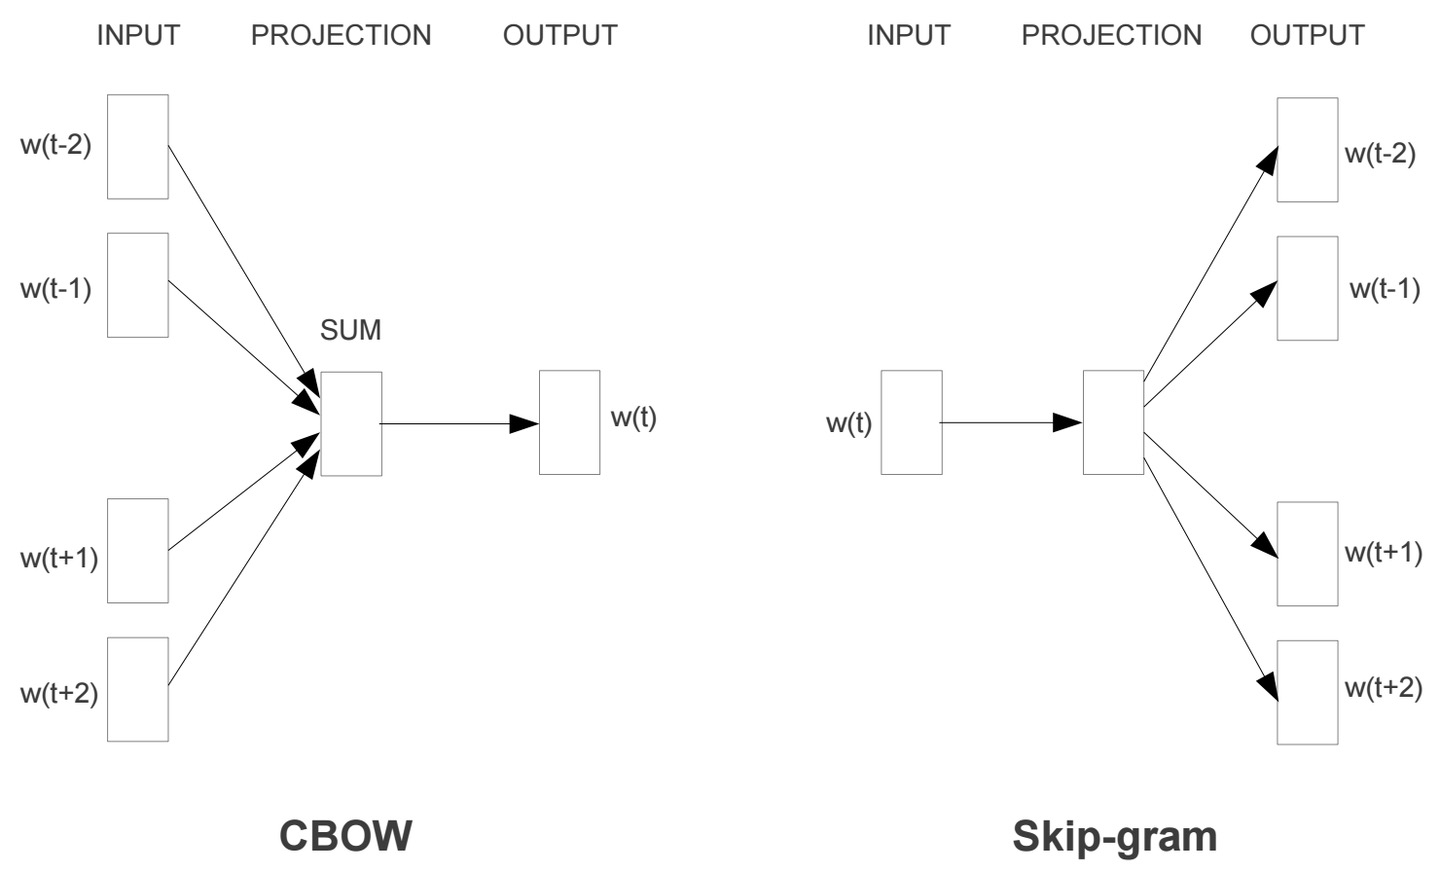
\includegraphics[width=1\textwidth]{images/word2vec.jpg} %插入图片,[]中设置图片大小,{}中是图片文件名
  \caption{CBOW vs Skip-gram对比原理图} %最终文档中希望显示的图片标题
  \label{Fig.word2vec} %用于文内引用的标签
\end{figure}

而本课题中用到的词嵌入算法就是Skip-gram,Skip-gram模型是输入一个单词,例如$x_t$输出是$\{x_{t-1},x_{t-2},x_{t+1},x_{t+2}\}$,上下文窗口大小为4。
举例来说的话,比如数据集中有个post为“China is a good country”。
如果将“a”作为训练的时候输入神经网络中的数据,则输出为单词组\{"China", "is", "good", "country"\}。

而如何得到词向量,仍然以“China is a good country”为例。

第一步输入向量,其为one-hot编码的向量,如果整个语料库数据集合中单词总数为10000,则集合中每个单词维度为词总数乘上一维,所以可以使用一个one-hot矩阵来表示"a",
然后隐藏层定300个神经元即可。如果规定为100个神经元,那么最后生成的权重矩阵的一个维度则为100。

然后在Input和Hide层之间,会存在一个维度为$(1*10^4)*(3*10^2)$权重矩阵,也可以称之为全部单词的词向量矩阵$W$。每个Input层的one-hot单词会在通过W之后变成一个大小为1*300
的矩阵,这也是该单词的词向量$V_c$。这个词向量会和$W^T$,也就是全部单词向量矩阵的转置矩阵进行相乘,之后会得到大小为$1*(10^4)$的矩阵,这个结果直观上理解就是输入单词和所有单词
的相似度,也可以理解为此单词出现时其他单词出现概率的合集。此时Output层输出的加权总数为10000个,然后通过softmax层将这10000个输出加权转换为等量的概率,
显然这10000个输出概率相加起来的和等于1,计算过程如图\ref{Fig.skipgram}所示。

\begin{figure}[htbp] %H为当前位置,!htb为忽略美学标准,htbp为浮动图形
  \centering %图片居中
  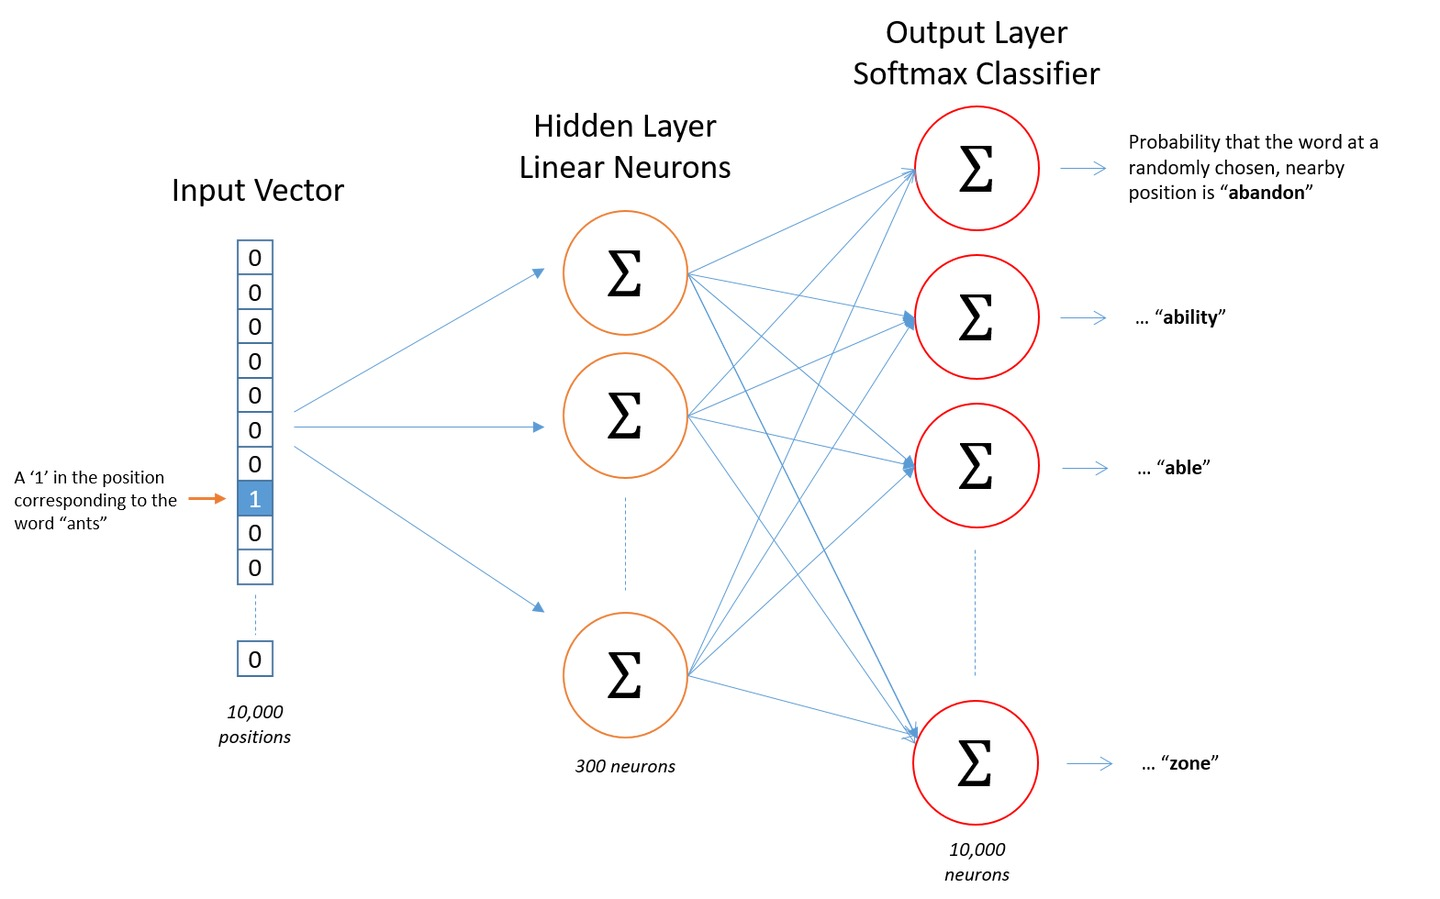
\includegraphics[width=1\textwidth]{images/skip-gram.png} %插入图片,[]中设置图片大小,{}中是图片文件名
  \caption{Skip-gram 原理图} %最终文档中希望显示的图片标题
  \label{Fig.skipgram} %用于文内引用的标签
\end{figure}

上述为skip-gram中全部的网络层示例。以"a"为例,如果将窗口大小window-size设置为2,即选用输入词语的前面两个单词和后面两个单词,
则一共会组四组训练数据,分别是(a,China)、(a,is)、(a,good)、(a,country)。

下面进行权重优化,拿(a,country)来说,"a"被展开为大小为$1*(10^4)$的one-hot向量矩阵,而经过Input层的预处理之后变为300维的词向量$V_{a}$,
经过隐藏层与softmax层之后输出为10000个概率分布,并且在后续反向传播中通过修正隐藏层的权重分布使得最后Output时$V_{a} * V_{country}^T$的大小提升。
代价函数(loss function)可以在训练过程中不断缩小两个矩阵的交叉熵,同样也可以实时计算出两个矩阵的损失值。通俗来说就是使得
这两个单词在向量空间的距离尽可能的近。

再通过不断重复的反向传播和迭代后,输入层和隐藏层在训练结束后会形成一个权重矩阵,矩阵的大小为10000*300,而最后求得的权重矩阵将会通过softmax层映射到
输入层中的单词向量,大小同样也为10000*300。

而业界也有许多开源的预训练词向量项目,例如\cite{wordvector},也是本课题中所使用到词向量集,因为本课题主要是设计一款闲聊机器人,所以使用到的为微博用户的发言数据,维度大小为300。


\subsection{循环神经网络}
循环神经网络,简称RNN\cite{mikolov2010recurrent},其基本思想是通过序列信息进行学习。在传统的神经网络里,Input和Output层是没有直接联系的,
然而如果需要预测句子中的一个单词是什么,则需要知道之前的word都有哪些。

如图\ref{Fig.rnn}为RNN单元展开图,之所以被称为循环网络,是因为它们对于句子里的每个元素会执行同样的任务,且输出会依赖于上一步的计算。
从另外一个层面来理解的话,RNN可以使用记忆来获得之前所有计算过的信息。
在按照时间步的序列展开RNN之后,可以在展开之后得到全部的序列网络,如果句中单词的总个数为10,神经网络就会被展开为10层。而RNN中每个Cell中的计算过程如下:

\begin{itemize}
  \item [1)] $x_t$:时刻t的输入,例如$x_2$则句子中的三号词的one-hot编码。
  \item [2)] $s_t$:时刻t的隐藏状态,也可以称为$h_t$,是网络的memory结构,$s_t$的计算表达式为:$s_t=f(Ux_t + Ws_{t-1})$
  \item [3)] $o_t$:时刻t的输出,也是所有的单词在下一个时刻出现概率的向量合集矩阵,表达式为$o_t = softmax(Vs_t)$
\end{itemize}

\begin{figure}[htbp] %H为当前位置,!htb为忽略美学标准,htbp为浮动图形
  \centering %图片居中
  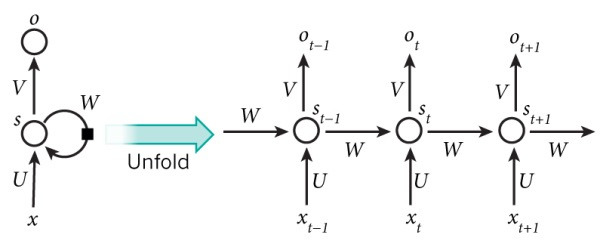
\includegraphics[width=0.8\textwidth]{images/rnn.png} %插入图片,[]中设置图片大小,{}中是图片文件名
  \caption{RNN展开原理图} %最终文档中希望显示的图片标题
  \label{Fig.rnn} %用于文内引用的标签
\end{figure}

此外在训练过程中需要注意以下几点。
\begin{itemize}
  \item [1)] 可以将隐藏状态$s_t$视为网络的存储器,获得先前时间中发生的信息,并且仅使用时间t处的存储器来计算输出。如前所述,这种情况稍微复杂一些,因为实际上只能获得一定时期的信息。
  \item [2)] 传统的神经网络在每个层中使用不同的参数,而RNN在所有步骤中都使用公共参数$(U,V,W)$,这意味着我们在每个步骤中执行相同的任务,但只有输入是不同的。这将减少需要学习的参数数量
  \item [3)] RNN最重要的就是隐藏层,它可以间接的用于获取句子的信息。图\ref{Fig.rnn}是不是绝对必要的,观察可以发现图中每个步骤都在输出,这需要针对不同的任务进行设计。例如,如果需要得到一个句子情感的预测结果,仅仅需要关注最终的输出而不需要
  关心每个单词的情感值。同样也不必每次都输入信息。
\end{itemize}

而RNN也有许多不同的种类来应对不同的需求。
\begin{itemize}
  \item [1)] one-to-one: 就是最普通的神经网络,几乎不能算是RNN。
  \item [2)] one-to-many: 常用于music generation、image captioning。
  \item [3)] many-to-one: 常用于sentiment classification。
  \item [4)] many-to-many (输入输出等长): 常用于video classification on frame level。
  \item [5)] many-to-many (输入输出不等长): 常用于machine translation,前一部分的作用是encoder,后一部分作用是decoder。
\end{itemize}

\subsection{序列到序列模型}
序列到序列(Sequence to Sequence)模型由两部分组成:Encoder和Decoder,每一个部分都是由一个RNN Cell结构,在本课题中
选择了GRU来作为RNN Cell子结构。传统的序列到序列模型,是通过Encoder把一个Sequence编码成为定长上下文向量$c$,然后Decoder再将
其解码为$y$,也就是输出的序列。而该模型,便是上一小节中提到的many-to-many可变长度结构的RNN模型,输入和输出序列是不等长的。
\begin{figure}[htbp] %H为当前位置,!htb为忽略美学标准,htbp为浮动图形
  \centering %图片居中
  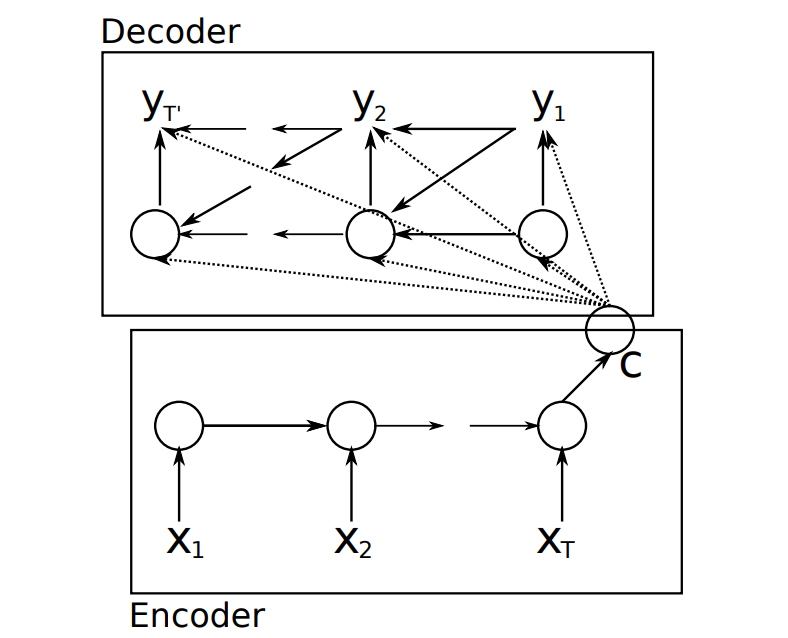
\includegraphics[width=0.6\textwidth]{images/seq2seq.png} %插入图片,[]中设置图片大小,{}中是图片文件名
  \caption{序列到序列模型原理图} %最终文档中希望显示的图片标题
  \label{Fig.seq2seq} %用于文内引用的标签
\end{figure}
这类框架由Cho\cite{cho2014learning}等人提出,同时Cho的团队也提出了GRU的原型。
如图\ref{Fig.seq2seq}所示,在Encoder中,主要关注的是隐藏状态$h_t$的生成,$h_t$的生成过程如\ref{1}所示:
\begin{align}
  h_t = tanh(W[h_{t-1},x_t] + b) \label{1}
\end{align}
最终Encoder输出上下文语义向量为\ref{2}所示:
\begin{align}
  &c = tanh(Uh_T) \label{2}
\end{align}
在Decoder中对$h_t$和$o_t$进行迭代计算。
\begin{align}
  &h_t = tanh(W[h_{t-1},y_{t-1},c] + b) \label{3}\\
  &o_t = softmax(Vh_t + c) \label{4}
\end{align}
而Decoder接收到Encoder传入的语义向量c之后,首先会输入$<START>$信号,和初始化$h_0$隐藏向量,然后按照公式\ref{3}和\ref{4}来进行循环计算。
\begin{align}
  &h_1 = tanh(W[h_0,y_0,c] + b)\notag\\
  &o_1 = softmax(Vh_1 + c)\notag\\
  &h_2 = tanh(W[h_1,y_1,c] + b)\notag\\
  &o_2 = softmax(Vh_1 + c)\notag\\
  &\dots\notag\\
  &h_t = tanh(W[h_{t-1},y_{t-1},c] + b)\notag\\
  &o_t = softmax(Vh_t + c)\notag
\end{align}
其中$o_t$是一个向量,是每个时间点的输出,向量的维度为单词表的长度。向量中每个值是每个单词的概率。
而这个过程将一直持续到预测值<END>的概率为最大时,预测就会结束。
预测下一个单词出现概率的公式如\ref{5}所示:
\begin{align}
  P(y_{t}|y_{t-1},y_{t-2},y_{t-3},\dots,y_{1},c) = g(h_{t},y_{t-1},c) \label{5}
\end{align}
从公式\ref{5}来说,其实不难发现所谓的对话生成模型,其实从根源上来说还是计算句子出现的概率,即当A句子出现时,B句子出现的概率为多大。
而最终生成出来的句子其实是出现概率最大的句子。


\subsection{注意力机制}
\begin{figure}[H] %H为当前位置,!htb为忽略美学标准,htbp为浮动图形
  \centering %图片居中
  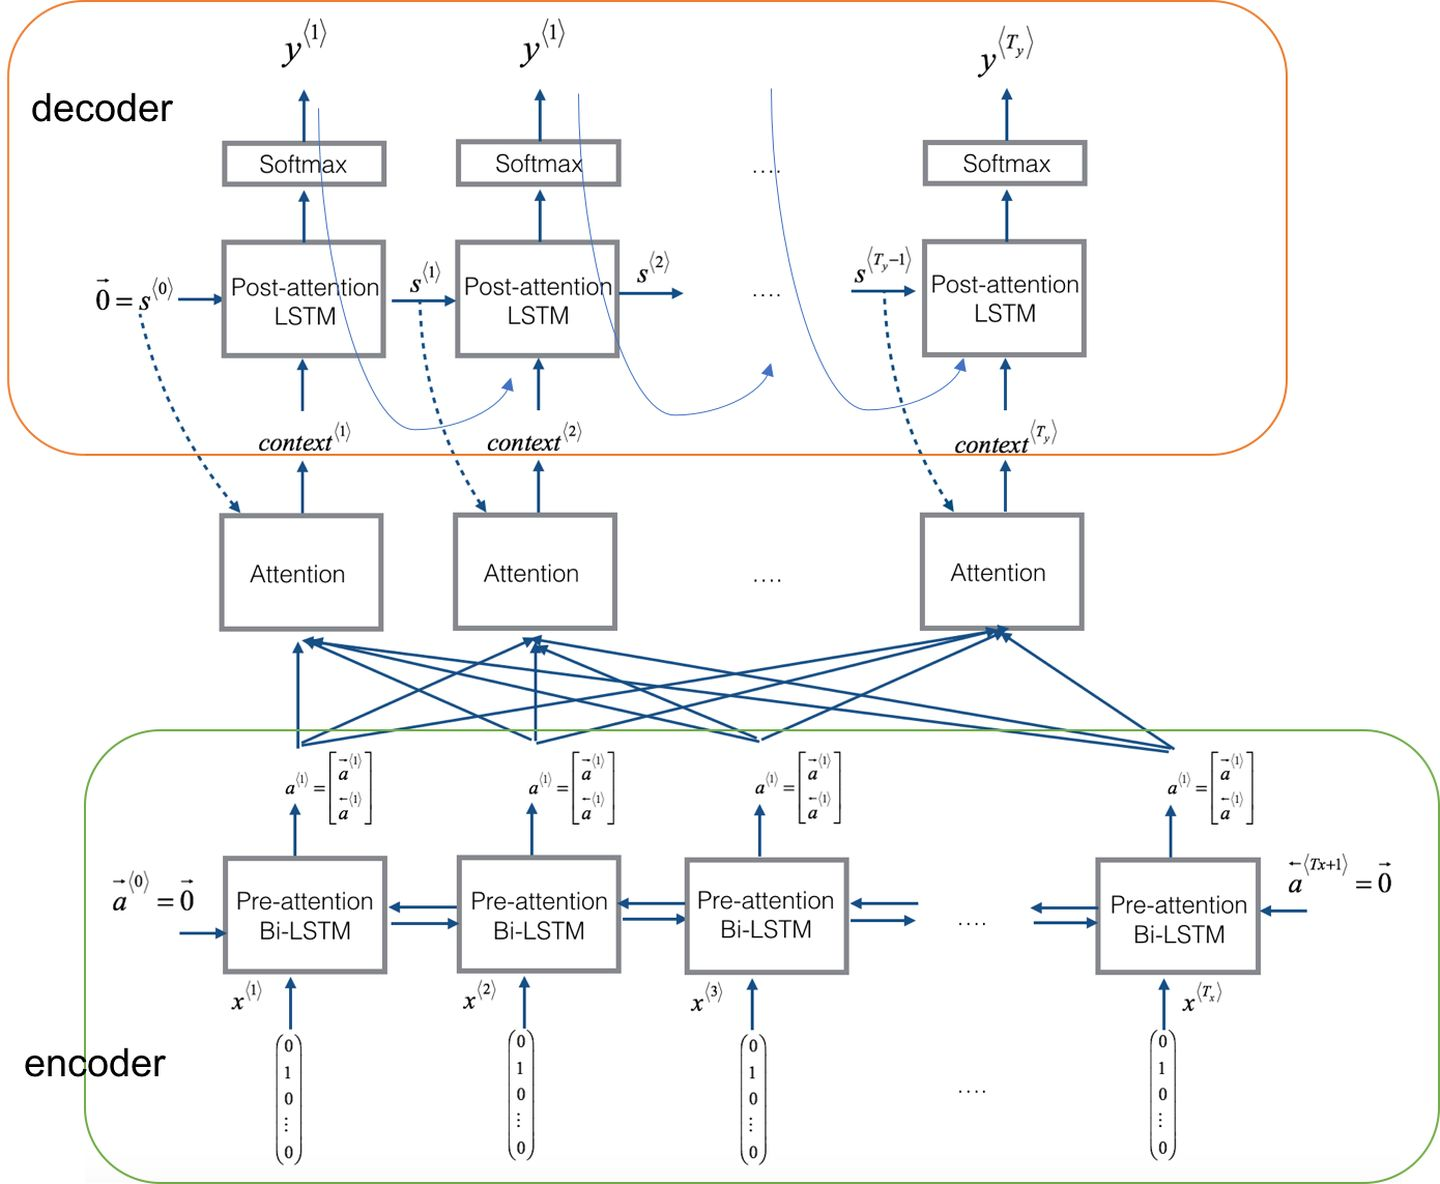
\includegraphics[width=0.9\textwidth]{images/attention.jpg} %插入图片,[]中设置图片大小,{}中是图片文件名
  \caption{Seq2seq with Attention原理图} %最终文档中希望显示的图片标题
  \label{Fig.attention} %用于文内引用的标签
\end{figure}
深入研究和剖析了序列到序列模型的机制和方法后会发现,在许多场景下传统Seq2seq方法会有很多局限性。
例如翻译一些很长的句子时,人工翻译时不会看完真个句子之后再进行翻译,而是先翻译一部分,然后再翻译进行下一部分,一直往复循环到最后。
因为记忆整个句子是不现实的,所以人工在翻译某个单词时,实际上只是把原来句子的局部范围最为上下文。所以attention机制就是
在针对每个所生成的$y_{t}$时,都会给出特定的context上下文信息$c_{t}$,这是非常符合人的直观感受的,这样原文中每个不同的部分对于翻译
当前的这个单词的影响权重是不一样的,这样效果就会大幅度提升,尤其是在解决翻译长难句的问题时。

如图\ref{Fig.attention}所示,和传统Seq2seq模型不同的是,Seq2seq with Attention实际上是在decoder和encoder之间加入了一个attention层。
用于计算每一步decode时所需要的上下文向量$context_t$。

decoder部分针对每种$y_t$进行计算的时候,包括三个部分的输入:
\begin{itemize}
  \item [1)]$context_t$:上下文信息。
  \item [2)]$h_{t-1}$:也可以写作$s_{t-1}$,为隐藏层状态。
  \item [3)]$y_{t-1}$:上个时刻中decoder的输出。
\end{itemize}

在attention模块部分,使用$A_{<t,t^*>}$来表示在翻译$y_{t}$的时候应该花在$a_{t^*}$上的注意力的数量,所以计算$context_{t}$:
\begin{align}
  context_{t} = \sum_{t^*=1}^{T_x}{A_{<t,t^{*}>}}a_{t^*} \label{6}
\end{align}
在attention进行计算时,输入包括两部分:
\begin{enumerate}
  \item [1)]decoder模块中上一个时刻的隐藏状态$s_{t-1}$。
  \item [2)]encoder模块所有时刻的输出$a_{t^*}$。
\end{enumerate}

如图\ref{Fig.attention}所示,attention模块其实本质上也是一个神经网络,然后使用softmax对输出进行归一化处理,如\ref{7}所示。
\begin{align}
  \sum_{t^*=1}^{T_x}{A_{<t,t^{*}>}}=1 \label{7}
\end{align}

\subsection{本章小结}
本个章节主要围绕本课题在设计实现过程中所需要用到的背景知识和技术来进行展开介绍,主要包括词嵌入、Seq2seq model以及模块Attention mechanism,但是和机器翻译不同的地方在于,本课题需要将情感纳入考量范围,
所以情感也作为一种特殊的语义参与输入和输出。首先本章节单独详细讲解了一下词嵌入的机制,因为词嵌入不仅是对语义的一种优化,也可以将其抽象思想应用于情感因素,
而具象出情感嵌入机制。接着是RNN模型的底层逻辑,RNN的诞生很好的解决了序列化信息处理难题,
其中最有名的应用则是Seq2seq模型,而Seq2seq模型也被称之为条件语言模型,因为在生成过程中,与其说是生成了一个句子,不如说是计算这个句子出现的概率是否是最大的。
而attention机制则是优化概率计算过程中权重分配的一个类神经网络层。而纵观本小节整个发展思路,其实就是在不断地模拟真人的思维方式,尤其是attention机制,不仅可以让机器关注于翻译时的
上下文,更可以聚焦于那些对情感有明显作用的词句,这也是本课题的中心思想。

\section{基于注意力机制的情感对话生成系统设计}
本章节将围绕整个原型系统的设计来展开,在Zhou\cite{DBLP:journals/corr/ZhouHZZL17}等人的课题基础上,加入了情感选择模块,并对基于内外部记忆的回复生成模块进行了优化改进,不再依赖于手动操作。

本课题主要围绕情感对话生成来开展工作,所以其主要任务是能主动获取post中的情感和语义,并预测出response中所使用的最佳情感并生成对应的回复。
\begin{figure}[H] %H为当前位置,!htb为忽略美学标准,htbp为浮动图形
  \centering %图片居中
  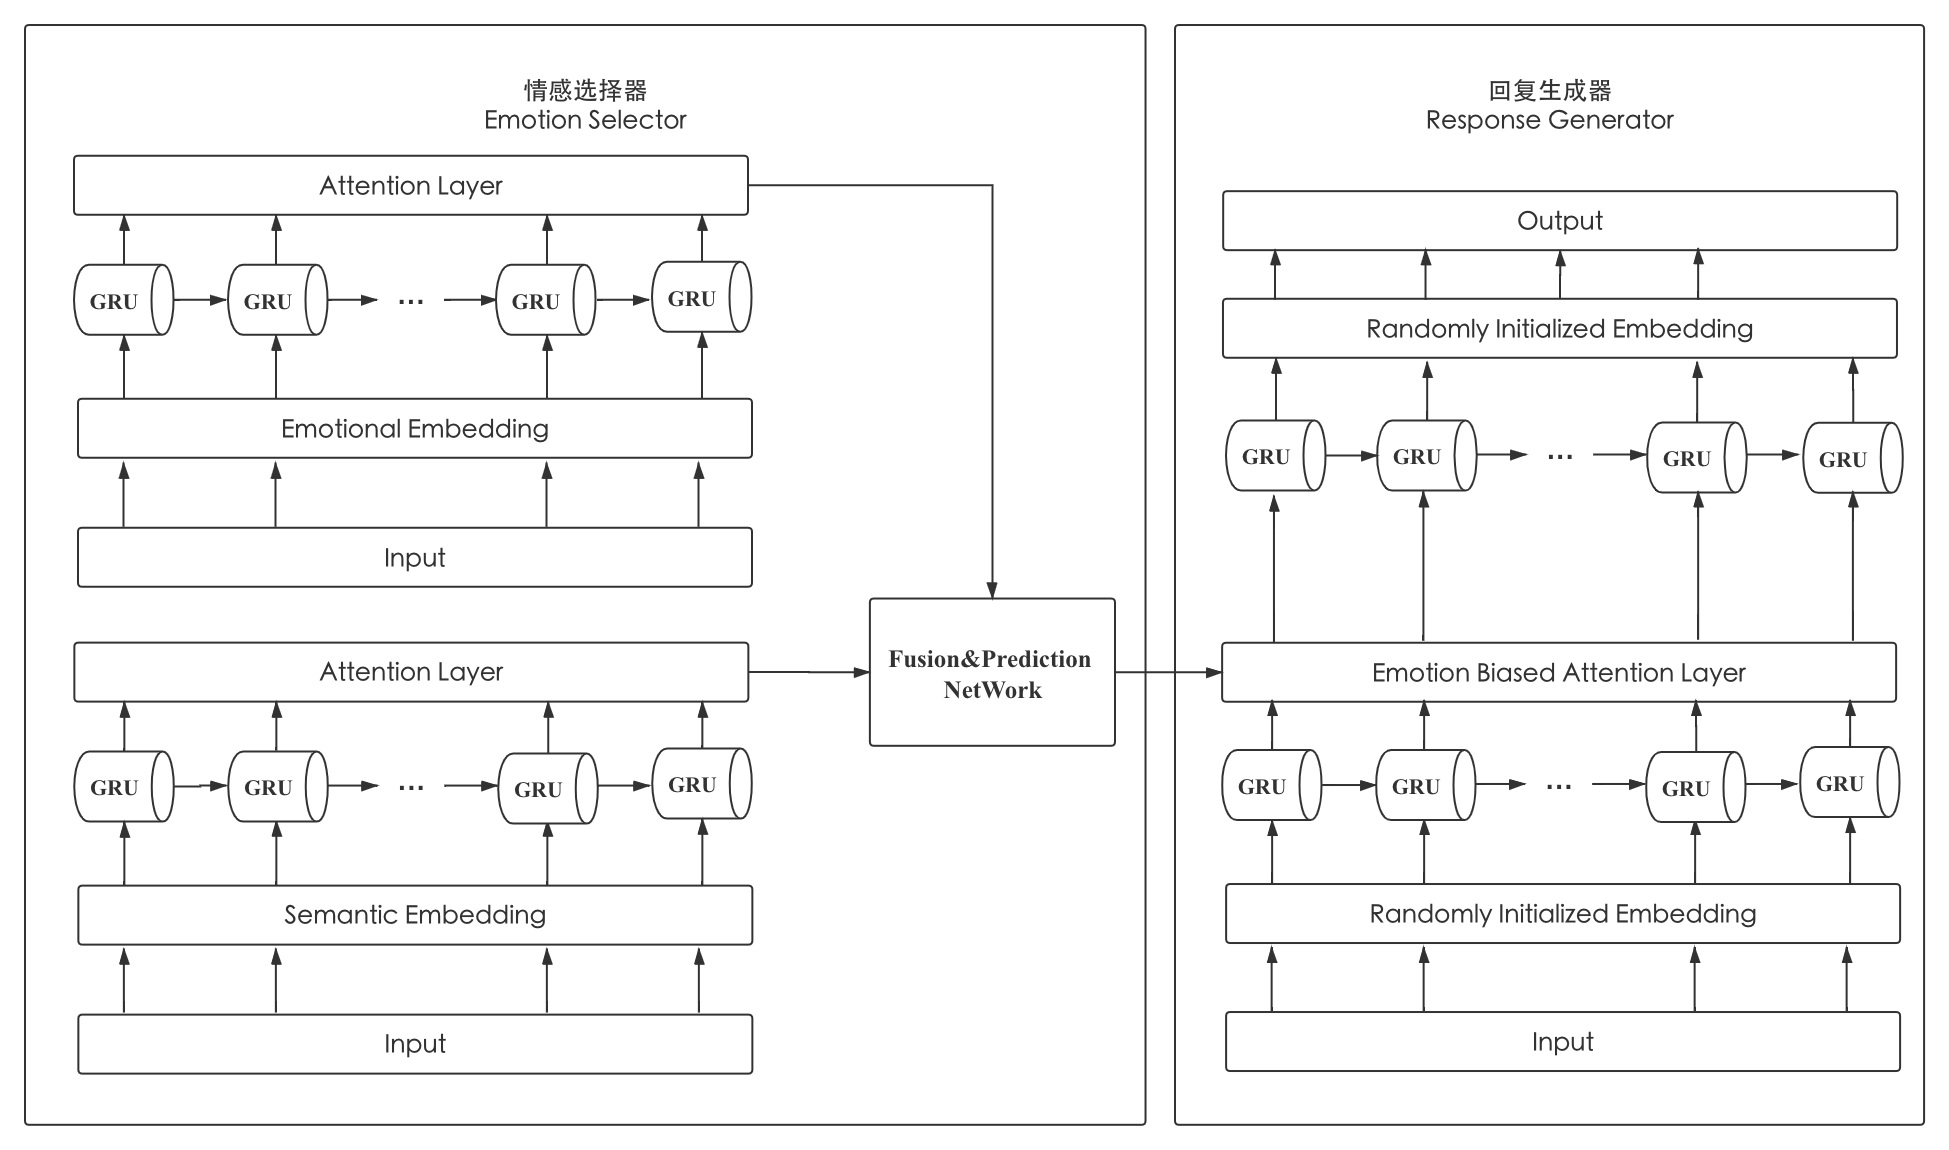
\includegraphics[width=1\textwidth]{images/ECMP.png} %插入图片,[]中设置图片大小,{}中是图片文件名
  \caption{Emotional Chat Machine Pro原理图} %最终文档中希望显示的图片标题
  \label{Fig.ECMP} %用于文内引用的标签
\end{figure}
综合需求可将系统的总体架构划分为情感选择模块和回复生成模块两个部分。系统命名为Emotion Chat Machine Pro,其在Zhou等人\cite{DBLP:journals/corr/ZhouHZZL17}的
基础上进行优化和功能升级,系统整体设计架构如图\ref{Fig.ECMP}所示。

情感选择模块可以拆分为情感序列编码、语义序列编码和融合预测,基于融合预测网络情感选择模块\cite{wei2019emotion}(Emotion Selector)使用情感编码模块,获取post中的感情倾向,
而语义编码模块则用于获取post中的语义向量,然后在融合预测网络中进行交叉计算。
而情感编码中使用情感嵌入、序列到序列(Seq2seq)模型以及注意力(Attention)机制,语义编码中同样也使用到了语义嵌入和基于注意力机制的序列到序列模型,所以很有意思的一点是,可以把情感也理解成为语义的一个维度。

而回复生成模块(Response Generator)则主要沿用ECM\cite{DBLP:journals/corr/ZhouHZZL17}模型中的生成模块,使用many-to-many不定长度的sequence to sequence模型来生成回复,
但是会在情感注意力层将情感选择模块所生成的向量纳入考量,其主要思想仍然是使用内部外部记忆来使得所选择的情感能在所生成的回复中得到完全的释放。

以下两个子章节为两个子模块的详细设计。

\subsection{基于融合预测网络的情感选择模块}
情感选择模块总共分为以下三个部分:
\begin{itemize}
  \item [1)]语义编码模块
  \item [2)]情感编码模块
  \item [3)]融合预测网络
\end{itemize} 
下面三个小节将分别描述这三个部分的功能和作用,以及训练时使用到的损失函数。其中融合预测网络会将语义编码模块和情感编码模块中所产生的语义和情感隐藏向量中进行权重重组融合,并得到最佳情感。

\subsubsection{语义编码}
针对于语义编码问题,输入为微博中用户对话的汉语文本,但模型只能接受数值型的数据输入,所以首先需要将输入句子进行语义嵌入。这里可以参考\cite{mikolov2013efficient}以及
\cite{wordvector}中词嵌入的详细论述,实现词嵌入目前的主流技术为Word2Vec,而本课题中采用了Skip-gram算法来从$post$中挖掘有效语义信息,并以向量的形式输入到GRU单元中进行计算。
从历史经验来看,使用300维来表示一个词语是最优解,且业界也已经有了很多比较成熟的实现方案和预训练好的结果。如果想用300个特征来定义一个单词(意思是每个单词可以被展开为一个300维的向量)。
那么一个大小为100万的词集最后在Word2Vec后的结果应该是一个1000000*300的矩阵。而最终的目标就是获得这个矩阵。从直觉上说,如果有两个不同的单词有着非常相近的上下文,例如:
\begin{shaded*}
  - 我爱中国

  - 我爱美国
\end{shaded*}


那么通过模型的训练,这两个单词(中国,美国)在词嵌入之后的向量应该非常相似。Word2Vec的创始人提出了几个非常重要的优化方案,
例如:
\begin{itemize}
  \item [1)]将非常常用的word当成单个单词进行处理。
  \item [2)]随机抽样出现次数非常高频的单词,这样的操作可以减少样本训练个数。
  \item [3)]对于所需要优化的目标,使用negative sampling来降低算力负担和提高训练词向量的质量。
\end{itemize}


在处理好输入之后,语义编码模块的神经网络层由基于注意力机制的Seq2seq模型所构成,而在本课题中,所采用的子单元(RNN Cell)
由GRU构成而并没有使用LSTM。

LSTM\cite{gers1999learning}(long short term memory)能从输入的词句数据集中习得长期的依赖关系。LSTM主要由四层构成,
第一层是遗忘层,它决定了cell中遗忘了哪些信息。第二层是记忆层,它决定了cell需要记忆哪些新的信息。第三层是更新层,它将cell遗忘和记忆的
内容拼接起来来更新cell的状态。第四层是输出层,决定了最后该输出什么,输出的值跟cell状态有关。此外LSTM网络还有一个巨大的优势
是攻克了梯度爆炸和消失的难题。

\begin{figure}[H] %H为当前位置,!htb为忽略美学标准,htbp为浮动图形
  \centering %图片居中
  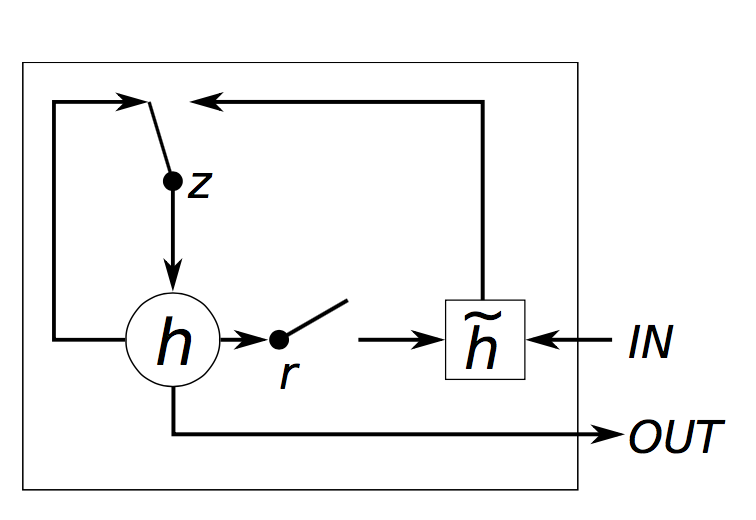
\includegraphics[width=0.5\textwidth]{images/GRU.png} %插入图片,[]中设置图片大小,{}中是图片文件名
  \caption{GRU 原理图} %最终文档中希望显示的图片标题
  \label{Fig.GRU} %用于文内引用的标签
\end{figure}

GRU\cite{dey2017gate}(Gated Recurrent Unit)结构上比LSTM简单,更重要的是它所消耗的计算资源要小的多。因为
GRU在实现过程中将记忆和遗忘合并到了同一个步骤中,GRU也是LSTM目前接受度和承认度最高的变体。
LSTM一共有三个门,分别是Input门、Forget和Output门。GRU如图\ref{Fig.GRU}所示,一共有Reset门和Update门两个门,
不难发现GRU并不会保留控制单元内部所产生的记忆并且摒弃了LSTM中的Output门。

梯度消失是RNN中一个非常棘手的问题,相较于LSTM的多个门来说,Reset门和Update门是GRU简化思想的经典之处。
这两个门可以决定哪些信息是可以作为最终的输出,它们可以保存跨度非常长的序列中的有效信息,并且这种信息不会随着时间的推移而清除或者被遗忘掉。
所以在本课题中采用了GRU而非LSTM来作为最小的RNN单元。

通过GRU网络,可以从$post$序列$x = (x_1,x_2,...,x_T)$中抽取关键信息,并且将其映射到隐藏层,计算公式如\ref{3.1}所示:
\begin{align}
  h_s^t = GRU(h_s^{t-1},x_t) \label{3.1}
\end{align}
其中$h_s^t$表示在时间t时隐藏层的状态。

但是为了增强隐藏层的信息传递有效性,可以使用注意力机制来使编码器更关注于和主题密切相关的词句。并且在最后获得最终的语义向量
$\widetilde{h_s}$,其计算公式如如\ref{3.2}所示:
\begin{align}
  \widetilde{h_s} = \sum_{i=1}^{T}a_i h_s^i \label{3.2}
\end{align}
如公式\ref{3.2}中所述,$a_i$是隐藏层状态向量$h_s^i$的权重,因为如注意力机制所描述的算法来说,$h_e^t$不再仅仅是依赖于$h_e^{t-1}$,
而是会依赖于每个GRU节点的隐藏层状态。而$a_i$则是训练过程中需要不断地去学习和重新分配的权重。

而$a_i$主要依赖于encoder的隐藏层状态$h_s^i$,将$h_s^i$输入一个多层感知机,然后再通过一个softmax层来得到$a_i$权重大小,并且可以确保的是
所有的$a_i$相加起来的总和为1。$a_i$的计算公式如\ref{3.3}所示:
\begin{align}
  a_i = softmax(V_a tanh(W_a(h_s^i)^T)) \label{3.3}
\end{align}
将输出全部映射到从0到1的区间内,softmax从本质上可以视为一种概率分布映射算法,从概率向量空间中的分布来多分类。它是常用于多分类的一个算法,
如果有一堆需要多分类的数,那么第i个元素的softmax的值如\ref{sfm}所示:
\begin{align}
  S_i = \frac{e_i}{\sum_j e_j} \label{sfm}
\end{align}
而tanh则是一个激活函数,激活函数在训练过程中是非常有必要的。因为如果使用线性的激活函数,那神经网络则失去了意义,仅仅是将输入经过线性组合变换之后
再输出,在这类情况下,多层隐藏层的神经网络和单个隐藏层的神经网络没有任何的区别,常用的激活函数一般有sigmoid、tanh和relu。在这里使用tanh作为激活
函数的原因是其值域为(-1,1),而sigmoid为(0,1),tanh的公式如\ref{tanh}所示:
\begin{align}
  a = g(z) = \frac{e^z - e^{-z}}{e^z + e^{-z}} \label{tanh}
\end{align}
但是sigmoid和tanh作为激活函数都有一些共同的缺点,比如z在很大或者很小的时候,梯度基本为0。所以在优化梯度下降算法来更新神经网络的时候使用tanh性能比较差,
但是在本课题中影响不大。因为z的分布一般位于中间值域。

综上在语义嵌入以及GRU网络编码之后,通过上述一系列转换,最终可以通过公式\ref{3.2}来获得最后的$\widetilde{h_s}$来作为语义编码向量。

\subsubsection{情感编码}
和语义编码类似的是,情感从抽象角度也是作为一种存在于语句中的信息,和主题一样通过可以被编码为向量。
同样输入为汉语文本,可以参考SSWE\cite{tang-etal-2014-learning}(sentiment specific word embedding)中的对推特的评论回复进行情感编码的实现过程来实现。
而本课题中可以模拟SSWE\cite{tang-etal-2014-learning}的算法来对中国微博中的用户评论回复来进行训练和编码。

情感作为一种信息,可以大致分类为$(like, disgust, sad, angry, happy, none)$6种情感。本课题中没有单一的采用一种情感来作为分类指标,而是将其将感情视作一种
多维数据,例如一句话的情感可以同时具有like和happy,或者sad和angry,如果的确只有单一的情感like,则为like和none的结合。而情感编码的本质其实就是计算不同词语对不同
情感的影响程度。如下面的例子,如果整个数据集只有这两句话:

\begin{shaded*}
    - 我爱中国

    - 她爱美国
\end{shaded*}

如果这两句话都被标记为like,那么在机器学习过程中,将判定“爱”对于like的影响程度是高于[“她,“吃”,“雪糕”]以及[“我”,“中国”]的权重。

同样在处理好输入sentiment embedding的相关问题后,将其输入GRU网络中进行训练。和语义编码不太类似的地方在于,情感编码在decode阶段是需要分类的,有
具体而准确的结果,所在本小节最后会根据此来设计损失函数。

同样的,情感编码也是通过GRU网络,从post序列$x = (x_1,x_2,...,x_T)$中抽取情感相关信息,然后映射到隐藏层,计算式如\ref{3.6}所示:
\begin{align}
  h_e^t = GRU(h_e^{t-1},x_t) \label{3.6}
\end{align}
其中$h_e^t$表示,隐藏层在时间t时候的状态。
如图\ref{Fig.attentionemotion}所示,$h_e^t$会在经过MLP和Softmax层之后得到一个权重$a_t$,其中采用到了多层感知机(MLP),也可以称作人工神经网络,多层感知机最大的特点就是层与层
之间都是全连接的,而传统的MLP可以分为输入层,隐藏层,输出层三层。当然,MLP的隐藏层可以分为很多层,这里视需求来进行选择。
\begin{figure}[!htb] %H为当前位置,!htb为忽略美学标准,htbp为浮动图形
  \centering %图片居中
  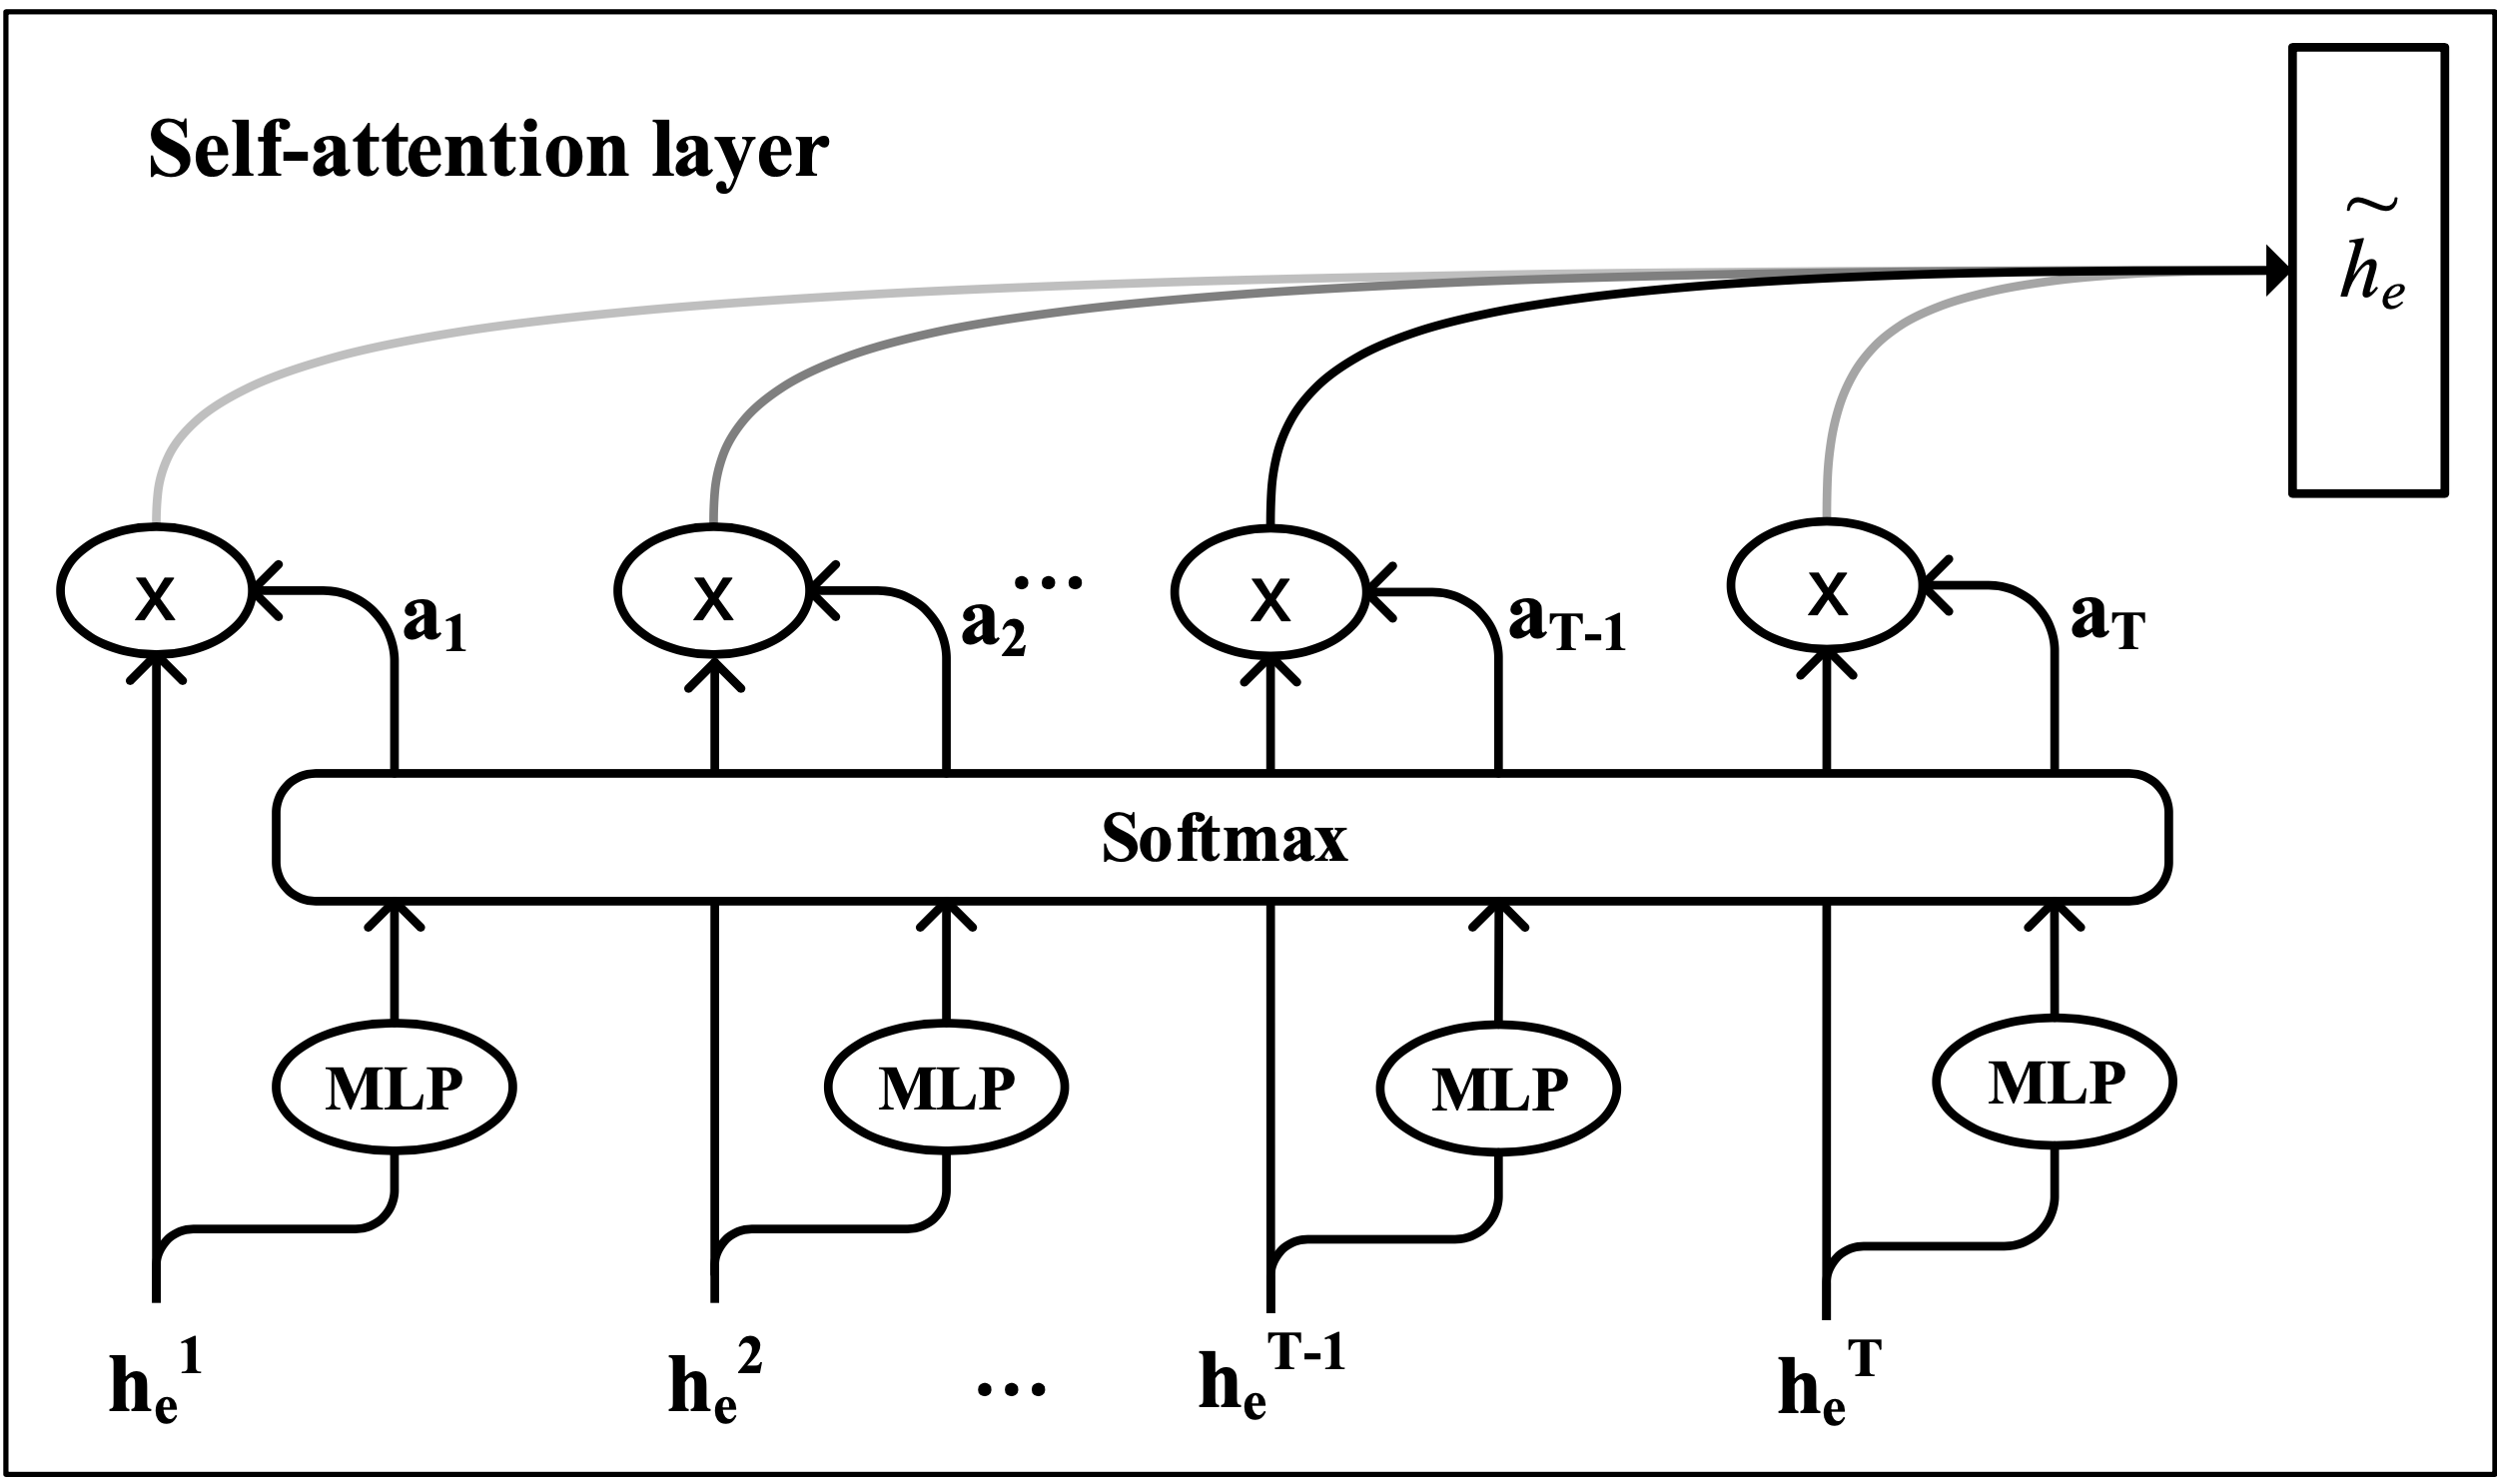
\includegraphics[width=1\textwidth]{images/attentionemotion.png} %插入图片,[]中设置图片大小,{}中是图片文件名
  \caption{attention layer原理图} %最终文档中希望显示的图片标题
  \label{Fig.attentionemotion} %用于文内引用的标签
\end{figure}

为了增强隐藏层对于情感信息的感知能力,如图\ref{Fig.attentionemotion},同样使用注意力机制来聚焦于情感词句,并在最后生成情感编码向量$\widetilde{h_e}$,
可知计算公式如\ref{3.7}所示:
\begin{align}
  \widetilde{h_e} = \sum_{i=1}^{T}a_i h_e^i \label{3.7}
\end{align}

整个网络为了使RNN网络其更注重于情感相关信息,设计了一个交叉熵损失函数。之所以这样做是因为,可以通过获取的$\widetilde{h_e}$来进行
计算,通过一个线性层和sigmoid层来将其映射情感空间中,来得到最后编码出来情感解码出来的结果的损失有多大。如公式\ref{3.8}和\ref{3.9}所示:
\begin{align}
  &\hat{e_p} = \sigma(W_e \widetilde{h_e} + b) \label{3.8}\\
  &\mathcal{L}_p = -e_p log(\hat{e_p}) \label{3.9}
\end{align}

通过损失函数的结果反向传播,然后经过上述转换后,最后可通过公式\ref{3.7}来得到最后的$\widetilde{h_e}$来作为情感编码向量。

\subsubsection{融合预测网络}
在经过情感编码和语义编码之后,需要将得到的两个向量进行融合并进行对response情感的预测,这也是本课题的重中之重。为了构建$e_r$的分类结果,
这里使用融合预测网络来融合均衡两个不同编码向量对于情感的贡献。并在之后部署一个预测网络来选择response的最佳情感分类。如图\ref{Fig.fusionnetwork}
所示,在将$\widetilde{h_s}$和$\widetilde{h_e}$输入一个sigmoid网络后可以获得一个权重大小。

\begin{figure}[htbp] %H为当前位置,!htb为忽略美学标准,htbp为浮动图形
  \centering %图片居中
  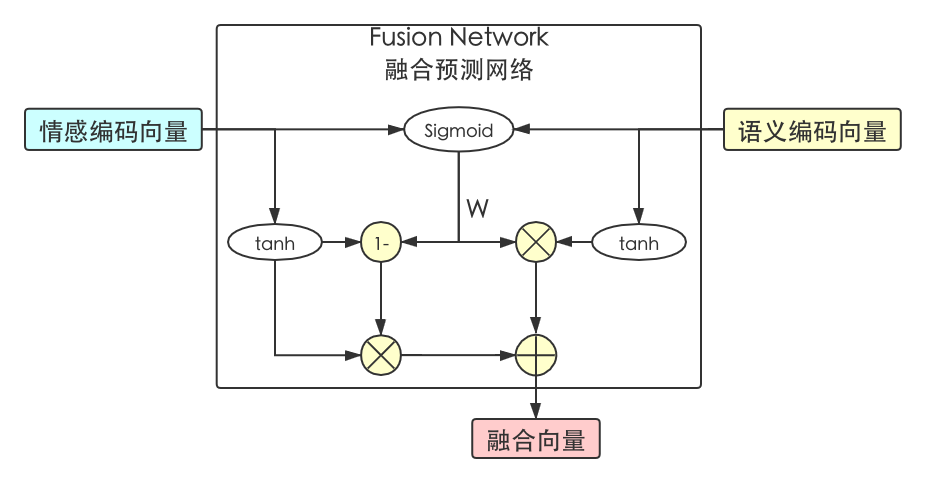
\includegraphics[width=1\textwidth]{images/fusionnetwork.png} %插入图片,[]中设置图片大小,{}中是图片文件名
  \caption{Fusion Network原理图} %最终文档中希望显示的图片标题
  \label{Fig.fusionnetwork} %用于文内引用的标签
\end{figure}
通过式\ref{3.10}来获取权重分布系数$w$,其实这个系数和GRU中用于记忆和遗忘的系数$z$有异曲同工之妙。
\begin{align}
  &w = \sigma([\widetilde{h_s};\widetilde{h_e}]) \label{3.10}
\end{align}
\begin{align}
  &{\widetilde{h_e^{'}}} = tanh(\widetilde{h_e}) \label{3.11}\\
  &{\widetilde{h_s^{'}}} = tanh(\widetilde{h_s}) \label{3.12}
\end{align}

之所以选用tanh作为激活函数的原因也很简单,衡量一个好的激活函数的方法是看其是否会在迭代训练中引发梯度消失或爆炸的问题,
反向传播时会对其求导,并与每一个layer进行相乘来计算误差。然而如果激活函数的导数比1要小,注意是绝对值,
在非常多的迭代相乘之后,误差的大小会无限接近于0。在Activation Function的导数的大于1时,同样也是绝对值,那么在非常多次的迭代相乘之后最后的结果会变得非常巨大,也就是与
梯度消失相对应的难题——梯度爆炸。


在得到这个最后被转换过的$\widetilde{h_s^{'}}$和$\widetilde{h_e^{'}}$之后,再通过如下公式进行融合求得最终权重:
\begin{align}
  {\widetilde{h_{es}}} = w \bigotimes {\widetilde{h_s^{'}}} + (1 - w) \bigotimes {\widetilde{h_e^{'}}} \label{3.13}
\end{align}
而拿到了$\widetilde{h_{es}}$之后,需要将其输入预测网络来产生一个情感向量,也就是$\hat{e_r}$。这里同样需要用到多层感知器
来进行一个映射。
\begin{align}
  \hat{e_r} = \sigma(W_r \widetilde{h_es} + b) \label{3.14}
\end{align}

通过上述公式可以直观的得到一个情感分类的概率分布。并且依据此来设计一个和公式\ref{3.9}类似的损失函数。
\begin{align}
  \mathcal{L}_r = -e_r log(\hat{e_r}) \label{3.15} 
\end{align}
这里的$e_r$是代表的每种情感是否会被选到,取值为0或者1,而$\hat{e_r}$则是选取到该情感的概率。最后情感选择器会将概率最高的emotion的类别输入到回复生成模块用于生成拥有最佳情感的回复。

\subsection{基于内部外部记忆的回复生成模块}
回复生成模块在ECM\cite{DBLP:journals/corr/ZhouHZZL17}中已经有了比较详细的设计,而在本课题中,为了能够融合语义和情感在生成的回复中,在ECM的基础进行改进和升级,以便能够接收在情感
选择模块中所产生的$e_r$,在其生成过程的主要思想如图\ref{Fig.ECM}依旧沿用了ECM中的内部外部记忆。
\begin{figure}[htbp] %H为当前位置,!htb为忽略美学标准,htbp为浮动图形
  \centering %图片居中
  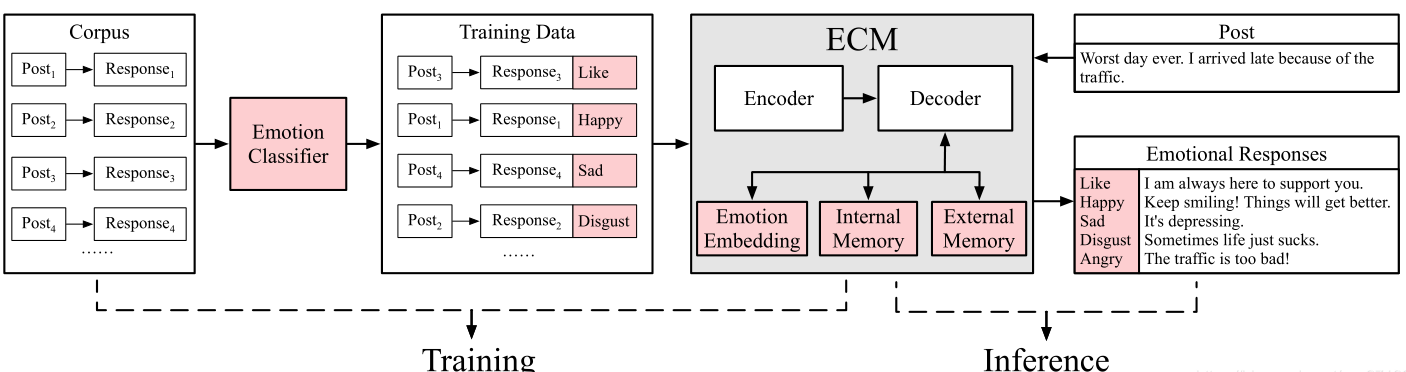
\includegraphics[width=1\textwidth]{images/ECM.png} %插入图片,[]中设置图片大小,{}中是图片文件名
  \caption{ECM原理图} %最终文档中希望显示的图片标题
  \label{Fig.ECM} %用于文内引用的标签
\end{figure}
而在本项目中继续沿用ECM中内外记忆的设计理念,因为内外情感的统一可以最大化的不损失语义的连贯性。

首先如Affect-Im\cite{ghosh2017affect}文中所述情感嵌入在生成的过程中是不会被改变的,但是这会极大程度的损失语义的连续性。从文中得到的启示是情感是快速波动且状态短暂的,
在生成情感回复时的情感变化过程也有着相同的特征,所以ECM动态捕捉每一步解码过程中的情感,并构建了一个基于内部记忆的模块来实现这个功能。

举个简单的例子来说明在表达情感时的整个过程,decode开始之前会存在一个情感状态存在于内在,并且在生成过程中的每一个step都会衰减,
所以在decode过程完成的时候情感状态已经为0,这也说明了该情感状态在生成回复时被非常充分的表达了出来。

ECM在最初的Seq2seq模型中加入了emotion embedding,这是一种静态方法,动态方法包括内部记忆情感状态网络以及外部记忆情感词语机制。这种改进能让ECM更准确的将输入的情感
类别转换为情感信息和情感状态并改写无情感的回复。

而下面将会详细的介绍基于内部记忆的情感状态网络模块的设计思路,以及基于外部记忆的情感词语选择器的基础理论。

\begin{figure}[H] %H为当前位置,!htb为忽略美学标准,htbp为浮动图形
  \centering %图片居中
  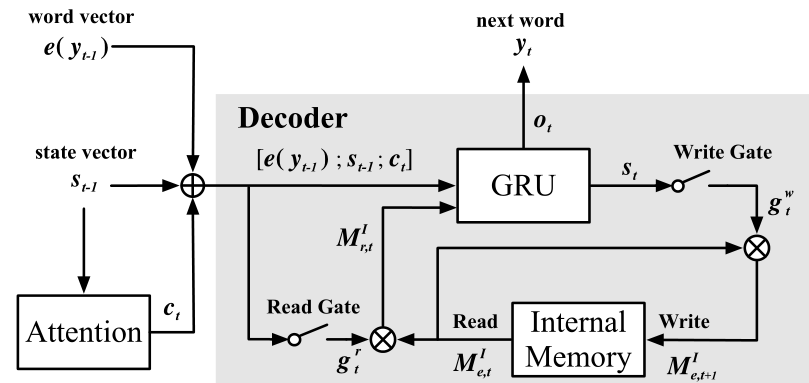
\includegraphics[width=0.7\textwidth]{images/imemory.png} %插入图片,[]中设置图片大小,{}中是图片文件名
  \caption{内部记忆模块原理图} %最终文档中希望显示的图片标题
  \label{Fig.imemory} %用于文内引用的标签
\end{figure}

如图\ref{Fig.imemory}所示,在内部记忆的解码模块中,内部情感状态变化和选词的关联不是显式的,所以并不能被直接的观察得到。在每个时间步的计算过程中,都会计算到Read Gate$g_t^t$
和Write Gate$g_t^w$,如公式\ref{rw}所示。
\begin{align}
  &g_t^r = \sigma(W_g^r[e(y_{t-1});s_{t-1};c_t])
  &g_t^w = \sigma(W_g^w[e(s_t)]) \label{rw}
\end{align}

$g_t^r$和$g_t^w$都是用于对内部记忆模块来读写的,在每个时间步中,$g_t^w$都会被消除一部分,而在最后一个时间步中情感状态会衰减至0,此时情感被完全表达。
\begin{align}
  &M_{r,t}^I = g_t^r \bigotimes M_{e,t}^I
  &M_{r,t+1}^I = g_t^w \bigotimes M_{e,t}^I
\end{align}
而隐藏层的状态也会根据内部情感状态来进行改变。
\begin{align}
  s_t = GRU(s_{t-1},[c_t;e(y_{t-1};M_{e,t}^I)])
\end{align}

情感表达和情感词并不是一个意思,比如可爱和令人仰慕,与一般的非情感词语相比,例如“中国”和“美国”,情感词承载了丰富的情感,
ECM通过为分别分配不同的生成权重给富含情感的词汇和普通非情感词,非隐式的构建回复生成中的情感表达的模型。基于此提出了外部记忆模块,
根据这一模型,生成过程中会从富有情感的词汇或普通的通用词汇中来选择生成词。

如图\ref{Fig.ememory},针对于不同词汇表达的不同情感,external memory模块会为情感词汇和普通无情感词汇分别赋上生成概率,来决策下一个单词如何生成。
此模块主要的思想是在每一个生成step中实时计算Emotion/Generic Word的权重,并且与internal memory模块强耦合。

\begin{figure}[H] %H为当前位置,!htb为忽略美学标准,htbp为浮动图形
  \centering %图片居中
  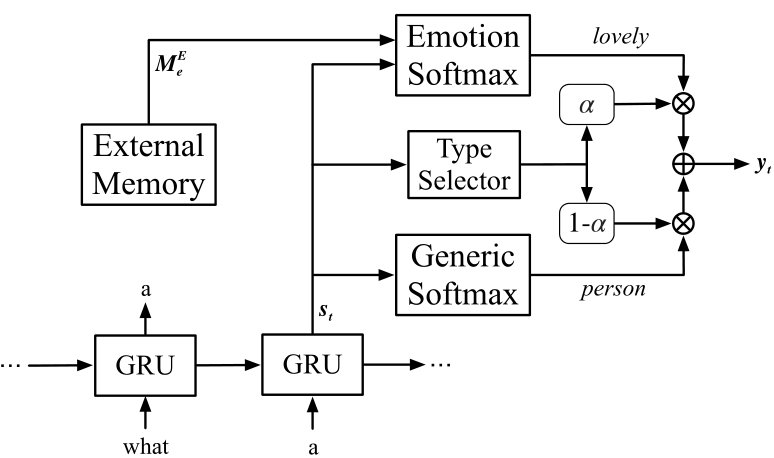
\includegraphics[width=0.7\textwidth]{images/ememory.png} %插入图片,[]中设置图片大小,{}中是图片文件名
  \caption{外部记忆模块原理图} %最终文档中希望显示的图片标题
  \label{Fig.ememory} %用于文内引用的标签
\end{figure}

\begin{align}
  &a_t = \sigma(v_u^T s_t)\\
  &P_g(y_t = w_g) = softmax(W_g^0 s_t)\\
  &P_e(y_t = w_e) = softmax(W_e^0 s_t)\\
  &y_t o_t = P(y_t) = a_t P_e(y_t=w_e) + (1-a_t)P_y(y_t=w_g)
\end{align}

以上描述的是在已知response的情感之后,生成对应回复的过程和方法,而现在需要设计response generator和emotion selector的衔接。
在获得了Emotion Selector给出的最佳回复情感之后,为了生成回复的情感嵌入向量,需要将$\hat{e_r}$的维度放大到和隐藏层向量一样大。
所以需要将$\hat{e_r}$乘上一个随机向量$W_e$。计算方法如\ref{3.16}所示:
\begin{align}
  V_e = W_e \hat{e_r} \label{3.16} 
\end{align}

引用Plutchik\cite{plutchik1980general}对情感的抽象本质的描述来说的话,现实生活中所描述的情感只是一维的,例如:like,sad等等,但是实际上人类在成长过程中,会不断地学习
这些情感所对应的场景以及本课题所提到的——词句。因此在这里随机输入的一个随机向量$V_e$就是相当于新生儿初次来到这个世界时,对于情感
的认知,它一定是不准确且需要不断地修正的,然后将其输入到RNN中,通过不断的反向传播来修正$V_e$的权重。

在本课题中整个数据集中包括大量无感情,单一情感和双重情感的post-response对。
在此前的ECM中,使用的是基于内在和外在记忆的模式,通过编码输入序列到RNN网络中来得到隐藏层向量$h = (h_1,h_2,...,h_T)$,然后
生成出一个上下文向量$c_t$用于decode这一步的隐藏层向量$s_t$。本课题将通过注意力机制重写这一过程,主要是优化了权重的分配这一步骤。
此前的计算方式如\ref{3.17}、\ref{3.18}、\ref{3.19}所示:
\begin{align}
  &u_i^t = v^T tanh(W_1h_i + W_2 s_t) \label{3.17}\\
  &a_i^t = softmax(u_i^t) \label{3.18}\\
  &c_t = \sum_{i=1}^T a_i^t h_i \label{3.19}
\end{align}

在每个时间t中,上下文向量$c_t$都会根据注意力机制重新编码,然后使得在长句子生成中拥有更好的性能。
但是以上的公式显然是忽略了刚刚所说到的$V_e$情感向量。现在,将其纳入训练算法中并依此重写公式\ref{3.17},如\ref{3.20}所示:
\begin{align}
  u_i^t = v^T tanh(W_1h_i + W_2 s_t + W_3V_e) \label{3.20}
\end{align}
然后通过公式\ref{3.18}和\ref{3.19}来生成全新的$c_t$。并且通过$c_t$和原先的解码器$s_t$融合产生新的隐藏层状态:
\begin{align}
  s^{'}_t = W_4[s_t;c_t] \label{3.21}
\end{align}
在获取到最新的隐藏层向量后,可以重构公式\ref{3.1}为\ref{3.22}:
\begin{align}
  s_t = GRU(s^{'}_{t-1},[y_{t-1};V_e]) \label{3.22}
\end{align}
上述计算式表示解码器在每次更新状态时,都会将上一轮的输出、隐藏层向量以及情感向量作为输入,这样可以最大化保持语义连贯和情感的饱满。

\subsection{损失函数}
在本课题中损失函数主要由两个部分构成,一个是情感损失,一个是语义的损失。可以表示为\ref{3.23}所示:
\begin{align}
  \mathcal{L}_{ECMP} (m) = a \mathcal{L}_e + (1-a)\mathcal{L}_{seq2seq} \label{3.23}
\end{align}

其中$a$是一个用来平衡情感损失和语义损失权重的因子,也是需要调参的一个地方。

而$\mathcal{L}_e$则是代表情感损失,计算过程如公式\ref{3.24}:
\begin{align}
  \mathcal{L}_e = \mathcal{L}_p + \mathcal{L}_r \label{3.24}
\end{align}
其中$\mathcal{L}_p$表示post中的情感损失,而$\mathcal{L}_r$表示response中的情感损失。

\subsection{设计中考虑的制约因素}
ECMP设计中的制约因素主要需要通过系统可用性、未来可扩展性、使用便捷性、算力资源预算四个角度来考察。
\subsubsection{系统可用性}
在整个原型系统的设计过程中,模块与模块之间的结耦合程度会极大的影响到整个系统的可用性,因为在理论上情感选择模块和回复生成模块是完全区分开来的
两个模块,但是实际的实现过程中,因为都是基于序列到序列模型来进行生成的,所以会出现大量的共用的函数,但是许多定制化的需求就会受到影响,并且在
设计过程中需要着重考虑的就是debug的成本,一个模块的异常会直接影响到另外一个模块,而且难以发觉是哪个步骤出现了问题。在设计实现完整个系统后,
也要不断的考虑异常情况,以免用户的非常规输入直接导致了系统的报错。

所以在不同的系统上和不同TensorFlow版本的兼容问题是设计过程中需要考虑的头号需求。

\subsubsection{模块可扩展性}
设计过程中比较重要的一点是该系统的可扩展性,因为本课题是基于ECM\cite{DBLP:journals/corr/ZhouHZZL17}的项目基础上进行进一步的扩展,而
为了使得后来的研究人员可以继续在本项目基础上做持续性的修改,模块之间的可扩展性也是非常重要的,因为可能后期有人需要在其基础上添加知识图谱、风格迁移等等
新的功能,所以在项目编写过程中不能把模型写的过于死板,并且一定要注意把注释写得更为详细以免后来者无法快速上手。但是可扩展性高也意味着系统的高度模块化,
这也会使得开发过程的效率会有所下降。

\subsubsection{使用便捷性}
因为本系统是基于TensorFlow编写的,所以在编写过程中需要考虑到的一点是,用户不可能直接通过命令行来与原型系统进行交互,并且原型系统在能正常运行之前,需要
配置大量的环境变量和安装包,这显然是非常反人类和不利于推广的。所以在后面的章节中也会提到,本课题基于Vue.js和Django框架设计了一套完整的交互界面供用户体验,
这套交互系统应该符合大众审美,且功能按钮齐全,交互界面简单明了,能让每个用户快速上手使用起来。

\subsubsection{算力资源预算约束}
因为本课题涉及到神经网络的训练,所以对CPU和GPU的配置都有一定的要求,在算力资源方面,因为最近的矿潮导致了GPU的全面涨价,所以在购买或者租赁算力时,需要考虑
训练过程中所需要使用到的算力资源消耗,以免超过预算。

\subsection{成本估算}

\subsubsection{基于Putnam模型的时间成本估算}
从开始设计项目到完成项目,以及前后调研和撰写代码的总时长来看,本次课题的时间成本大约为3个月左右。
代码设计的实际实际约为4周,而代码实现的实际时间大约为4周,其余时间主要用在学习相关理论知识和对接课题组成员,本节采用
Putnam模型\cite{王红珍2012软件开发成本估算模型的研究}来估算整个软件开发的成本。

而Putnam提出的动态多变量模型,计算过程如下。
\begin{align}
  L = Ck * K^{1/3} * td^{4/3} \notag
\end{align}

\begin{generaltab}{Putnam系数}{tbl:putnam}
  \begin{tabular}{c|ccc}
    \toprule
    类型 & 开销大小 \\
    \midrule
    L(源代码行数) & $1573$(行) \\
    K(整个开发过程所花费时间) & $0.75$(年)\\
    Td(开发持续时间)& $0.25$(年)\\
    Ck(技术状态常数)& $11000$ \\
    \bottomrule
  \end{tabular}
\end{generaltab}
如下表\ref{tbl:putnam}所示,本项目Ck值位于优秀队列,作为一个规模较小的深度学习项目,该项目的实现成本并不高,所以可移植性和可拓展性均较强。
而项目的主要人力资源都用在了前期的相关知识学习和系统架构实现部分。

\subsubsection{算力资源与硬件消耗的资金成本}
因为此次课题是有关于深度学习的项目,所以主要的开销在电脑硬件和电力消耗上。
\begin{generaltab}{成本开销}{tbl:hmm}
  \begin{tabular}{c|ccc}
    \toprule
    类型 & GPU & CPU & 其他硬件 \\
    \midrule
    电脑硬件 & $1350¥$ & $2700¥$ & $17000¥$ \\
    电力消耗 & $20¥$ & $5¥$ & $10¥$ \\
    \bottomrule
  \end{tabular}
\end{generaltab}
因为硬件是之前已经采购过的,所以真实的硬件开销应该只需要计算折旧的部分,大约为硬件开销的5\%左右。


\subsection{本章小结}
本章的主要内容是围绕情感对话系统来进行展开,所以主要分为情感选择器和回复生成器的设计。

在情感选择器部分中着重需要注意的是情感嵌入(sentiment embedding)以及attention机制的引入,这两个部分也是主要工作量的来源,从本质上说情感嵌入也是语义嵌入
的一个维度,只不过在本课题中将其单独进行抽象和具象编码,而情感选择器中的语义嵌入则更类似于传统机器翻译模型中编码器的结构,除此之外,
融合网络将情感编码$\widehat{h_e}$和语义编码$\widetilde{h_s}$后的结构进行权重分配,这里的设计其实类似于GRU Cell的内部记忆/遗忘门的实现,
并将分配之后得到的向量映射到情感空间来得到response的最佳情感,这里分配重组后向量的损失函数是反向传播时考虑的重要因素,也会在训练时不断更新。

对于回复生成器的设计则更多的参考了ECM\cite{DBLP:journals/corr/ZhouHZZL17}的设计,在解码阶段采用内部情感状态衰减和外部情感词语选择两个模块,内部情感状态会不断地衰减以防对语义连贯性产生过大的影响,而
外部情感词语选择则在每一步生成词的过程中,选择情感丰富的词或者非情感相关普通词。这样生成出来的response在语义流畅度上有着更好的表现,且完全不需要再依赖于人来手动
进行选择回复的最佳情感。

\section{基于注意力机制的情感对话生成系统实现}
在本课题的实现过程中,主要采用python作为编码语言,因为python本质上是一种解释型语言,而且面向对象,最重要的是
其生态链中有着大量实用的第三方库。现如今在深度学习方面,TensorFlow和PyTorch已经是最为流行的两个用于深度学习的库了。
而在本课题中采用的则是TensorFlow来作为项目基础框架。

而因为要使用到GPU的原因,所以使用的训练环境如下:
\begin{itemize}
  \item 系统环境:Windows 10
  \item 编码平台:PyCharm
  \item GPU配置:GTX 1050Ti
  \item TensorFlow Version:tensorflow-gpu==0.12.*
  \item Python Version:3.5
\end{itemize}

\subsection{系统主体架构实现}
系统的主体虽然是分为情感选择和回复生成两个部分,但是从传统的机器学习项目上来说,总体结构依然是分为数据处理、训练、测试三个主要部分的。

系统在Train和Test阶段中,都会经历数据准备(prepare data)和模型建立(create model)两个步骤,
而数据准备阶段的主要实现过程包括读取数据、数据序列化以及特定格式嵌入,模型部署则是对基于attention机制的Seq2seq的引用,除了数据嵌入层不同以外,其他大同小异。
如图\ref{Fig.main}所示。
其中值得注意的是,为了更好的进行情感向量的嵌入,实验过程中将改写多种GRU Cell变体来适应新的需求,比如内部情感状态记忆功能或者外部情感词权重分配能力。
而Response Generator的实现则沿用了ECM的实现过程,在本章中将会对其
算法实现过程进行详细的剖析。
\begin{figure}[H] %H为当前位置,!htb为忽略美学标准,htbp为浮动图形
  \centering %图片居中
  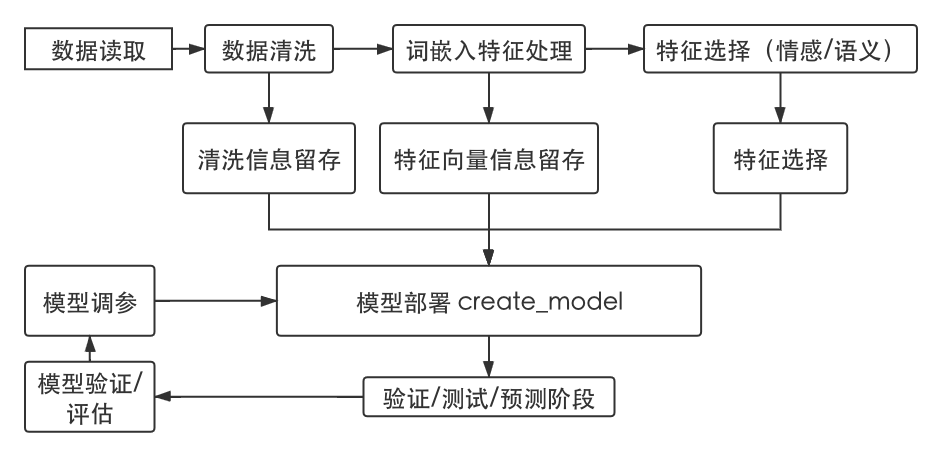
\includegraphics[width=1\textwidth]{images/main.png} %插入图片,[]中设置图片大小,{}中是图片文件名
  \caption{系统主体框架} %最终文档中希望显示的图片标题
  \label{Fig.main} %用于文内引用的标签
\end{figure}

\subsubsection{数据处理}
在本次实验中采用的是Emotional Short-Text Conversation(ESTC)数据集,其中包括了400万条微博中现实存在的对话,原始数据集大小为4,433,949条$post-response$对。
因为考虑到训练时间和成本的大小,最终选用了100万条数据来进行训练。而ESTC数据集来源于STC数据集,该数据集由尚老师团队整理和提供,其中包括了大量的情感对话,但是STC的
原始数据不包括情感标签,所以在这里采用BERT算法为其进行自动打标。而每一句话最终的情感打标结果为一个情感对如[like,happy],即包含两种情感而非单一的情感。

首先,定义ESTC的数据集的每条数据结构如下:
\begin{shaded*}
    {ESTC Data Set:A standard format}
    \begin{align}
    [post, emotion 1, emotion 2],[response, emotion 1, emotion 2]\notag
    \end{align}
\end{shaded*}

首先将数据将会被分为训练集、验证集、测试集三个部分。如图\ref{Fig.data}
\begin{figure}[H] %H为当前位置,!htb为忽略美学标准,htbp为浮动图形
  \centering %图片居中
  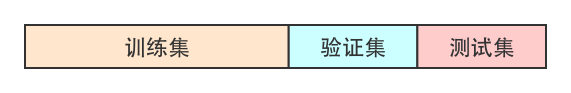
\includegraphics[width=0.8\textwidth]{images/data.png} %插入图片,[]中设置图片大小,{}中是图片文件名
  \caption{数据集划分} %最终文档中希望显示的图片标题
  \label{Fig.data} %用于文内引用的标签
\end{figure}
数据集合划分和处理的伪代码如算法\ref{alg:ppd}所示:
\begin{algorithm}
  \caption{prepare data for train/test/dev}
  \label{alg:ppd}
  \begin{algorithmic}
    \Input{$filedata$}
    \Output{$train;dev;test set$}
    \State split filedata to trainset/devset/testset
    \For {$traindata \in trainset$}
      \State $tokenizer(traindata)$
    \EndFor
    \For {$devdata \in devset$}
      \State $tokenizer(devdata)$
    \EndFor
    \For {$testdata \in testset$}
      \State $tokenizer(testdata)$
    \EndFor
  \end{algorithmic}
\end{algorithm}


在准备数据阶段,需要将每一条数据转换成为RNN可以理解的格式,主要包括数据初始化,统计词频
以及word embedding,以训练集为例,首先会将训练集中的每条数据单独抽取出来分为post和response两个大的集合,因为post和response中的映射关系不一定是相同的,为了
避免两者互相干扰,所以将其分开来分别统计,而在编码阶段如果遇到不存在于词库中的单词,则直接使用<UNK>来作为它的编码
。之所以用词频来为单词重新编号,是因为原生的单词并不能直接被输入网络之中,所以在这里用词频来作为网络的输入。注意这里是
最简单的一种词嵌入方式one-hot,并且仅有一个维度的信息。

如果在预训练阶段已经给出了训练好的word embedding vector,那么直接读取相应的文件就可以了,并且按照逐个的单词来分别进行word embedding,需要注意的是在进行此操作时
需要注意是通过语义还是情感来进行词嵌入,在tokenizer阶段,也包括了对数据的清洗,将一些非常短或没有实际意义的文本清洗去掉,因为这些内容会非常影响最后的训练效果,并且没有
任何的实际含义,在海量的对话中也不乏大量的反人类语言。tokenizer结构如算法\ref{alg:tok}所示:
\begin{algorithm}
  \caption{tokenizer算法}
  \label{alg:tok}
  \begin{algorithmic}
    \Input{$trainset$}
    \Output{$refinedata$}
    \For {$sentence \in trainset$}
      \State Initialize vocabulary for post//构建post词库
      \State Initialize vocabulary for response//构建response词库
      \State Add $<PAD> <UNK> <EOS> <GO> $ to post/response set
    \EndFor
    \For {$sentence \in trainset$}
        \State $sentence =  enumerate(sentence)$//词频转换
        \State $sentece = wordembedding(sentence)$
    \EndFor
  \end{algorithmic}
\end{algorithm}

\subsubsection{模型建立}
模型建立阶段也称为create model,在整个过程中属于顶部结构,不论是训练还是测试,首先都需要基于GRU的RNN网络来创建模型。
\begin{itemize}
  \item Read TensorFlow basic setting
  \item Choose data category(sentiment/semantic)
  \item Load post/response word embedding data
  \item Create model finished
\end{itemize}
\begin{algorithm}
  \caption{create model}
  \label{alg:crm}
  \begin{algorithmic}
    \Input{$session$}
    \Output{$model$}
    \State $model = Seq2seqModel(basic Setting)$
    \If{$checkpoint != none$}
      \State $model.restore(session,checkpoint)$
    \Else \State $model.initialize(session)$
    \EndIf
  \end{algorithmic}
\end{algorithm}


上述中描述了ECMP中的两个通用模块的主要思路,下面将根据第三章中的设计思路,ECMP分为情感选择器(Emotion Selector)和回复生成器(Response Generator)来分别进行实现。
因为两者都是基于Seq2seq with Attention的模型,所以在GRU网络的实现上采用了相同的结构,而没有进行强行的结耦合。

\subsection{基于融合预测网络的情感选择器}
Emotion Selector的中心思想为情感嵌入和语义嵌入,因为情感和语义都属于语言中的信息,只是属于不同的维度,所以
可以将其在抽象层面视为同一种信息。这里首先需要搭建好GRU Cell来构建RNN网络。首先针对于预测网络搭建一种多维GRU Cell来帮助抽取情感
信息和语义信息。因为预测网络中的解码部分不包括语句生成(只需要输出最终隐藏层向量),所以不用考虑内外部记忆的实现,只需要基于原生的
RNNCell搭建多维GRUCell结构即可。

\begin{algorithm}
  \caption{Multiple GRU Cell}
  \label{alg:mtgc}
  \begin{algorithmic}
    \Input{$GRUCell, number_{layer}$}
    \Output{$Input_{current}, State_{current}$}
    \State $GRUCells = GRUCell * number_{layer}$
    \For{$cell \in GRUCells$}
      \State $Input_{current}, State_{current} = cell(Input_{current}, State_{current})$
    \EndFor
  \end{algorithmic}
\end{algorithm}

在构建好多维GRU Cell之后,需要实现attention部分并且将其封装进语义/情感编码模块中,所以接下来只需要分别为情感编码和语义编码部分实现封装部分即可。
\begin{itemize}
  \item [1)]embedding encoder with attention(semantic)
  \item [2)]embedding decoder with attention(semantic)
  \item [3)]embedding encoder with attention(sentiment)
  \item [4)]embedding decoder with attention(sentiment)
\end{itemize}

其中embedding attention seq2seq函数则是对encoder和decoder的封装,情感编码模块以及语义编码模块共用这一模块且输入输出流
格式完全一致,在获取到输出的$\widetilde{h_s}$和$\widetilde{h_e}$之后,通过公式\ref{3.13}进行向量层面的权重融合,
如算法\ref{alg:fusionprediction}所示。
\begin{algorithm}
  \caption{Fusion Prediction}
  \label{alg:fusionprediction}
  \begin{algorithmic}
    \Input{$\widetilde{h_s},\widetilde{h_e},\widetilde{h_{es}}$}
    \Output{$e_r$}
      \State 向量通过激活函数激活阶段
      \State $w = sigmoid([\widetilde{h_s};\widetilde{h_e}])$
      \State ${\widetilde{h_e^{'}}} = tanh(\widetilde{h_e})$
      \State ${\widetilde{h_s^{'}}} = tanh(\widetilde{h_s})$
      \State 向量融合阶段
      \State ${\widetilde{h_{es}}} = w \bigotimes {\widetilde{h_s^{'}}} + (1 - w) \bigotimes {\widetilde{h_e^{'}}}$
      \State 根据$\widetilde{h_{es}}$进行response情感预测
      \State $e_r = MLP(sigmoid(\widetilde{h_{es}}))$
  \end{algorithmic}
\end{algorithm}

\subsection{基于内部外部记忆的回复生成器}
Response Generator则如设计部分中所说,沿用了ECM\cite{DBLP:journals/corr/ZhouHZZL17}的设计模块,项目中
通过重构了带有内部记忆能力的GRU单元来搭建generate单元,以便于生成指定情绪的回复。

\subsubsection{情感状态类别嵌入}
在选择最佳的回复情感之后,必不可少的是情感状态类别的嵌入,情绪状态会被当作一种语句中的附加信息被传入Emotion biased Attention层。
根据情感类别$e$,在经过random initialize之后得到$\boldsymbol{V}_e$,之后会将这个随机向量传入RNN网络中进行训练。
分别将词嵌入向量$\boldsymbol{e}(y_{t-1})$、情感类别嵌入向量$\boldsymbol{V}_e$以及context向量$\boldsymbol{c}_t$一起传入编码器用于更新
它的隐藏层状态$\boldsymbol{s}_t$。
\begin{align}
  \boldsymbol { s } _ { \boldsymbol { t } } = \mathbf { G } \mathbf { R } \mathbf { U } \left( \boldsymbol { s } _ { t - 1 } , \left[ \boldsymbol { c } _ { t } ; \boldsymbol { e } \left( y _ { t - 1 } \right) ; \boldsymbol { V } _ { e } \right] \right) \notag
\end{align}

而基于获得的$\boldsymbol{s}_t$,解码器所计算得到的概率分布将会通过\ref{3.20}来计算,来生成下一个$y_t$。

\subsubsection{内部情感存储器实现}
在解码开始时,情感状态处于顶峰,因为此时还没有开始生成回复,所以情感状态完全没有衰减。但在之后的每个step中,情感状态都会根据当前状况衰退一定的量,以免影响到语义通顺,
内部情感存储器的实现如图\ref{Fig.imemory}所示。

经过每个step步骤$t$时,response generator会读取上一步中解码的单词$\boldsymbol{e}(y_{t-1})$的word embedding格式数据,
根据解码器在上一步状态$\boldsymbol{s}_{t-1}$以及当这一步的context向量$\boldsymbol{c}_t$,将这两者作为传入数据去得到Read门状态${\boldsymbol{s}_t^r}$。

Write门状态$\boldsymbol{g}_t^w$依赖于解码器此时的状态$\boldsymbol{s}_t$。如下为读取和写入门的算法实现:
$$\boldsymbol { g } _ { t } ^ { w } = \operatorname { sigmoid } \left( \mathbf { W } _ { \mathbf { g } } ^ { \mathbf { w } } \boldsymbol { s } _ { t } \right)$$
$$\boldsymbol { g } _ { t } ^ { r } = \operatorname { sigmoid } \left( \mathbf { W } _ { \mathbf { g } } ^ { \mathbf { r } } \left[ \boldsymbol { e } \left( y _ { t - 1 } \right) ; \boldsymbol { s } _ { t - 1 } ; \boldsymbol { c } _ { t } \right] \right)$$

读写门可以利用TensorFlow中已经实现的RNNCell来重构GRUCell以便于其支持内部记忆。这里命名为MEMGRUCell,如算法\ref{alg:mgc}所示:
\begin{algorithm}
  \caption{MEM GRU Cell}
  \label{alg:mgc}
  \begin{algorithmic}
    \Input{$emotion, imemory, state, imputs, number_{units}$}
    \Output{$new_h$}
    \State 传入初始情感状态
    \State $params.append(emotion,imemory)$
    \State 获取Reset gate和Update gate的初始状态
    \State $r, u, c = arrayops.split(linear(params, 3 * number_{units}))$
    \State Reset gate 和 Update gate转换
    \State $r, u = arrayops.split(linear([inputs, state], 2 * number_{units}))$
    \State $r, u = sigmoid(r+r_{old}), sigmoid(u+u_{old})$
    \State Candidate输出层
    \State $c = activation(c+linear([inputs, r * state], number_{units}))$
    \State 获取最新的隐藏层向量
    \State $new_h = u * state + (1 - u) * c$
  \end{algorithmic}
\end{algorithm}

而和基于融合预测网络的情感预测模块相同的是,这里也用到了多维GRUCell来提高信息的捕获能力,如算法\ref{alg:mtgc}所示。

紧接着将写入和读取门分别作用域内部存储器中。在每个step中,情绪状态会衰退一定的值(通过$\boldsymbol{g}_t^w$)。

在最后一个step中,内部情感存储器的情感会缩减为0。整个步骤的的算法实现如下:
$$\boldsymbol { M } _ { r , t } ^ { I } = \boldsymbol { g } _ { t } ^ { r } \otimes \boldsymbol { M } _ { e , t } ^ { I }$$
$$\boldsymbol { M } _ { e , t + 1 } ^ { I } = \boldsymbol { g } _ { t } ^ { w } \otimes \boldsymbol { M } _ { e , t } ^ { I }$$

其中,$\otimes$表示元素乘,$r/w$分别表示为读和写,$I$表示内部状态码。

在上述过程中,GRU状态将不断被更新$\boldsymbol{s}_t$根据此前的target单词$\boldsymbol{e}(y_{t-1})$,
此前的解码器state$\boldsymbol{s}_{t-1}$和此时的context文向量$\boldsymbol{c}_t$和情感状态一起来更新$\boldsymbol{M}_{r,t}^I$,定义如下:
$$\boldsymbol { s } _ { t } = \mathbf { G } \mathbf { R } \mathbf { U } \left( \boldsymbol { s } _ { t - 1 } , \left[ \boldsymbol { c } _ { t } ; \boldsymbol { e } \left( y _ { t - 1 } \right) ; \boldsymbol { M } _ { r , t } ^ { I } \right] \right)$$

基于状态$s_t$,可以获得单词在向量空间中生成的分布$\boldsymbol{o}_t$,
然后可以依据此过程采样下一个单词$y_t$,在生成下个单词后,$\boldsymbol{M}_{e,t+1}^I$将会被写回到内部情感存储器中,在不断的读出和写入之后情感会衰减为0,
因为不难发现$0 \leq \operatorname { sigmoid } ( \theta ) \leq 1$。

这种操作十分类似于人类记忆或者内存网络中的DELETE\cite{miller1956human}。

\subsubsection{外部情感词汇选择器实现}
外部情感词汇选择器的主要功能是在每一步的生成过程中,选择是具有情感倾向的词语还是普通词汇。根据图\ref{Fig.ememory}所示,
选择器向量$\alpha_t$分别计算出富含情感或者通用词的生成概率。
然后计算两个概率串联的结果,最后采样所生成的下一个单词$y_t$,实现过程如下:
\begin{align} 
  \alpha _ { t } \notag
  &= \operatorname { sigmoid } \left( \mathbf { v } _ { \mathbf { u } } ^ { \top } \boldsymbol { s } _ { t } \right) \ P _ { g } \left( y _ { t } = w _ { g } \right) \\\notag
  & = \operatorname { softmax } \left( \mathbf { W } _ { \mathbf { g } } ^ { \mathbf { o } } \boldsymbol { s } _ { t } \right) \ P _ { e } \left( y _ { t } = w _ { e } \right) \\\notag
  & = \operatorname { softmax } \left( \mathbf { W } _ { \mathbf { e } } ^ { \mathbf { o } } \boldsymbol { s } _ { t } \right) \ y _ { t } \sim \boldsymbol { o } _ { t } = P \left( y _ { t } \right) \\\notag
  P \left( y _ { t } \right) 
  &= \left[ \begin{array} { c } \left( 1 - \alpha _ { t } \right) P _ { g } \left( y _ { t } = w _ { g } \right) \ \alpha _ { t } P _ { e } \left( y _ { t } = w _ { e } \right) \end{array} \right] \notag
\end{align}

其中,$\alpha_t \in [0,1]$只是标量,这里用于平衡过程选择中通用词$w_g$和情感词$w_e$的权重分配,
\begin{itemize}
  \item $P_g/P_e$:分别表示为通用无情感词和富含情感词的概率
  \item $P(y_t)$:最后得到的生成句子的向量概率分布
\end{itemize}
需要注意的是这两个词汇表一定是没有交集的,最终所生成的分布$P(y_t)$则是两个分布概率向量的串联。

\subsection{本章小结}
本个章节从算法级别描述了整个系统的实现模式。也从侧面印证了ECMP模型对于ECM\cite{DBLP:journals/corr/ZhouHZZL17}的主要提升在于情感选择器的实现。其中不论是情感选择还是回复生成,本质上来说都是序列到序列
的生成,而算法实现的角度上来看也都是基于seq2seq框架来进行编码解码,本章的重点是混合预测网络的应用以及word embedding的加入,非常显著的加快了神经网络的训练速度并且
优化了训练效果。并且相较于此前的所有情感对话生成模型来看,ECMP不再将依赖于人工手动选择回复的最佳情感,而是完全依赖于Emotion Selector的判断。在下一个章节,
将会论证ECMP的语义流畅度和情感准确度,保证其在自动选择情感的前提下,不会损失过度的语义逻辑和主题相关性。

\section{性能评估与分析}
\subsection{测试环境与方案}
因为开发机平台为macOS,所以测试环境系统也选用了macOS平台,测试的硬件软件环境如下:
\begin{itemize}
  \item [1)]System Version:macOS Big Sur 11.2 Beta版
  \item [2)]PyCharm Version:2019.3.3
  \item [3)]TensorFlow Version:tensorflow-gpu==0.12
  \item [4)]Python Version: 3.5
\end{itemize}

根据Liu\cite{liu-etal-2016-evaluate}等人的论文可知BLEU并不适用于评估对话生成等课题。
从机器自动评估角度上来说,因为BLEU并不会考虑语言表达上的精准度,且测评精度经常会受到常用词的干扰。
所以在本课题中使用了Li\cite{li2015diversity}等人的评估方法,即使用$distinct 1$和$distinct 2$来对对话生成的多样性进行评估。
这个评估方式通过计算生成语句中的一元语法和双元语法的数量来判断生成response的质量,并且这个指标
从侧面也可以印证情感的多样性。

然后从人工评估角度上来说,这里从数据集中随机抽取了200条post,然后输入以下四种对话生成系统中来进行评估
\begin{itemize}
  \item [1)]Seq2seq:传统的序列到序列模型,没有进行词嵌入
  \item [2)]Seq2seq-emb:包含词嵌入的序列到序列模型
  \item [3)]ECM:Emotion Chat Machine,不包括自动情感选择模块
  \item [4)]ECMP:Emotion Chat Machine Pro,也就是本次课题模型
\end{itemize}
从以上四个模型得出的response集合,会被分配给4位非本课题研究领域的同学来进行人工打分,从语义和情感准确度两个角度来为其
进行打分,而从情感准确度的角度上来说,如果response所生成的情感非常不准确,例如出现了即开心又难过的情感对,则会被标记为0分,
此外将会被标记为1分。而综合来说,一句话的质量由情感准确度和语义流畅度所组成,如公式\ref{5.1}所示:
\begin{align}
  \mathcal{Q}_{response} = S_{sentiment} \cup S_{semantics} \label{5.1}
\end{align}
其中$S_{sentiment}$代表了$response$的情感得分,$S_{semantics}$则代表了语义得分,如果其中之一得到了1分,那么直接将该条$response$的综合评分标记为1分。

在评估开始之前,根据实验结果最终选择了第59000个step时的结果。此时的$response$预测结果最为准确,如图\ref{Fig.59000}所示,此时的
损失值已经基本不再下降,而预测的$response$情感的准确度也达到了最高。

\begin{figure}[H] %H为当前位置,!htb为忽略美学标准,htbp为浮动图形
  \centering %图片居中
  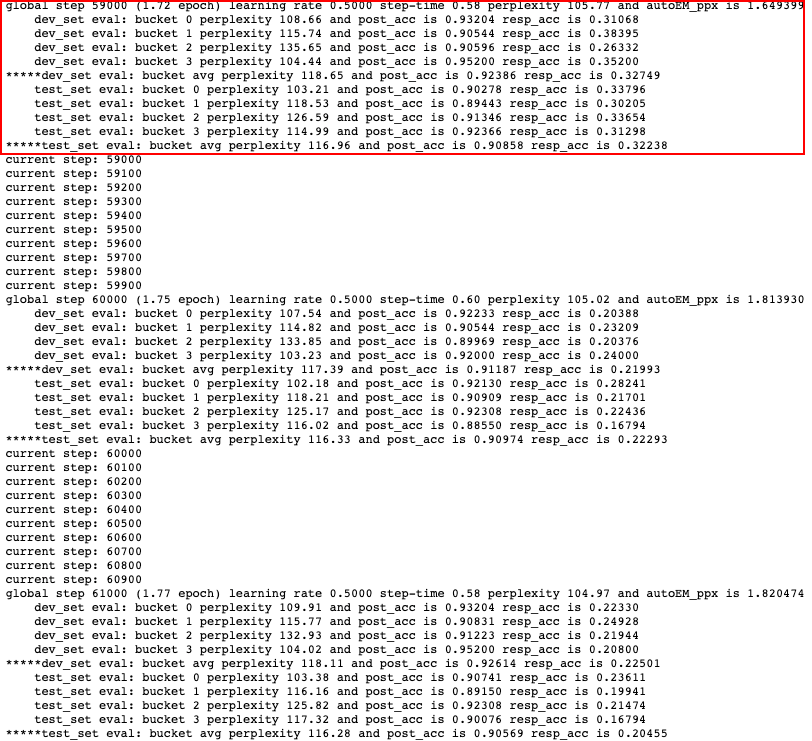
\includegraphics[width=1\textwidth]{images/59000.png} %插入图片,[]中设置图片大小,{}中是图片文件名
  \caption{59000Step Accuracy} %最终文档中希望显示的图片标题
  \label{Fig.59000} %用于文内引用的标签
\end{figure}

\subsection{自动评估}
将选取的200个$post$,分别传入四个模型(Seq2seq,Seq2seq-emb,ECM,ECMP)中,来得到对应的$response$。
如图\ref{Fig.result}所示,下图为ECMP中所自动生成的$response$结果集。
\begin{figure}[H] %H为当前位置,!htb为忽略美学标准,htbp为浮动图形
  \centering %图片居中
  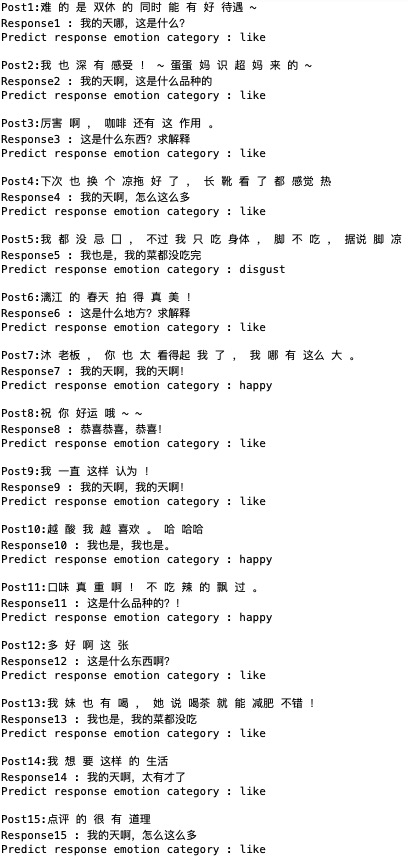
\includegraphics[width=0.6\textwidth]{images/result.png} %插入图片,[]中设置图片大小,{}中是图片文件名
  \caption{ECMP测试集生成结果} %最终文档中希望显示的图片标题
  \label{Fig.result} %用于文内引用的标签
\end{figure}

\begin{generaltab}{机器自动评估结果}{tbl:aer}
  \begin{tabular}{c|ccc}
    \toprule
    模型类型 & Distinct-1 & Distinct-2 \\
    \midrule
    ECMP & $0.0713$ & $0.2503$\\
    ECM & $0.0551$ & $0.2022$\\
    Seq2seq-emb & $0.0628$ & $0.2370$\\
    Seq2seq & $0.0608$ & $0.2104$\\
    \bottomrule
  \end{tabular}
\end{generaltab}

如表\ref{tbl:hmm}所示,Seq2seq和Seq2seq-emb在语句生成的多样性上的效果要略好于ECM,原因可能是在ECM的结构中包括了情感融入,这会限制语义的多样性,
在生成回复时可以选择的词汇变得更少,而不具有情感倾向的模型则可以有更多的选择性。

而ECMP模型针对这一点进行了比较大的优化,主要是在ECMP摒弃了单情感的约束,而是将情感分布在整个向量空间中,所以在语义多样性上,其表现要略好于其他三个模型。
虽然ECMP目前来说已经在语义多样性上优于各大模型,但是因为没有加入知识图谱,所以在生成的回复上略显单一,这也是后期工作中所需要进一步进行突破的地方。


\subsection{人工评估}

\begin{generaltab}{人工评估结果}{tbl:her}
  \begin{tabular}{c|ccc}
    \toprule
    模型类型 & $S_{semantics}$ & $S_{sentiment}$ & $Q_{response}$\\
    \midrule
    ECMP & $0.415$ & $0.885$ & $0.390$\\
    ECM & $0.355$ & $0.870$ & $0.310$\\
    Seq2seq-emb & $0.280$ & $0.795$ & $0.250$\\
    Seq2seq & $0.390$ & $0.815$ & $0.360$\\
    \bottomrule
  \end{tabular}
\end{generaltab}
从表\ref{tbl:her}来看,Seq2seq-emb的表现最差,这也是意料之中的。因为该模型在生成过程中被不恰当的使用到了词嵌入,导致生成了比传统Seq2seq模型更晦涩难懂的句子。

传统Seq2seq更多的时候只是对$post$换了一种说法改写后阐述出来,所以人工评判可能会觉得$response$生成的情感和语义都比较符合当前的语境和情感,但是显然这种回复是含金量并不高的。

而ECM模型则取得了相对来说不错的成绩,但是因为ECM无法自动选择最佳情感,所以在这里只能默认ECM的$response$采用和$post$一致的情感,这显然是非常有局限性的,因为没有人希望在愤怒或者伤心
的表达时,听到对方同样的回复同样也是愤怒伤感的。而ECMP则分别从语义丰富度和情感准确度两个角度分别对模型进行了优化,使得ECMP所生成的语句有了较好的效果。
\begin{figure}[H] %H为当前位置,!htb为忽略美学标准,htbp为浮动图形
  \centering %图片居中
  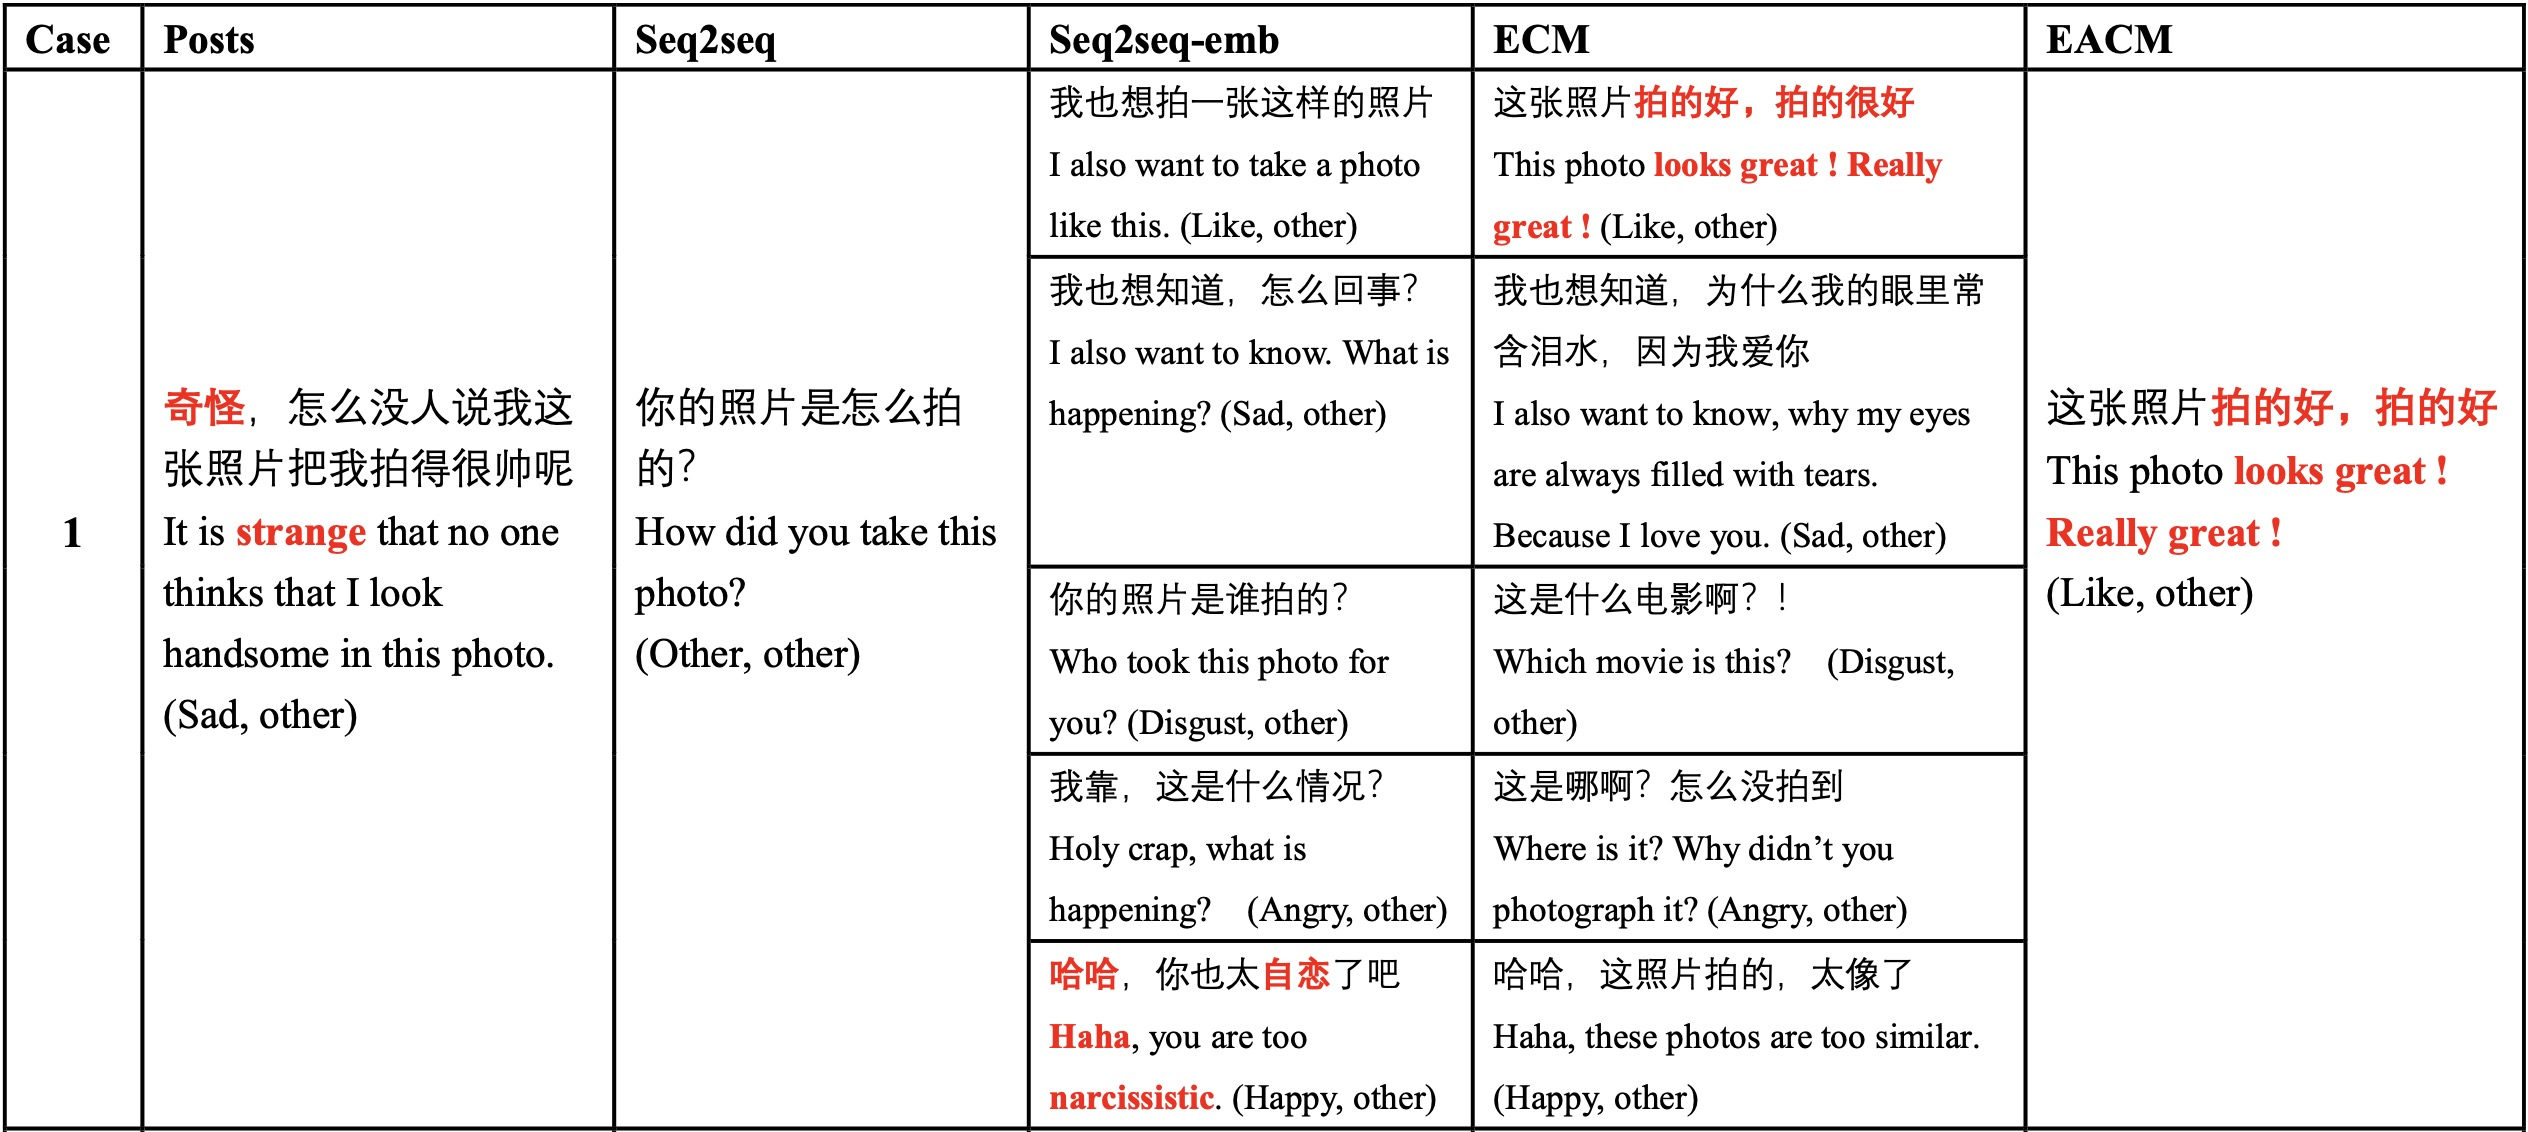
\includegraphics[width=1\textwidth]{images/4models.png} %插入图片,[]中设置图片大小,{}中是图片文件名
  \caption{四类模型对比图} %最终文档中希望显示的图片标题
  \label{Fig.4models} %用于文内引用的标签
\end{figure}
而图\ref{Fig.4models}则是一种对于现有四种模型分别在同一个$post$下所生成的$response$的示例。

\subsection{系统界面}
因为用户直接在IDE中直接进行交互的体验感并不是很好,而且对于系统的环境配置非常繁琐,所以在完成了原型系统的设计后,希望能有一个更为便捷的交互系统来进行直观的展示,
所以本项目采用了Vue.js来作为前端,而Django作为后端来进行交互系统的设计,其中蚂蚁金服团队提供了一套非常完善的前端套件Ant Design of Vue来让开发者快速开发自己的展示平台,
所以本项目也是通过这个平台来进行可视化交互界面的设计。虽然Django也有其前端界面,但是其开发效率太低,所以不予使用。

ECMP平台的前端设计模块中包括用户登陆、结果分析和对话互动三个主要模块。
\subsubsection{用户登陆页面}
用户登陆界面主要使用了异步校验法,因为没有引入数据库结构所以账号密码直接写死在代码数据结构中。而后端在接收到前端传来的account和password字段之后,会和正确的字段进行校验,
如果成功,则分配相应的用户权限并跳转至对话页面,如果失败则直接通过悬浮气泡进行提示。
\begin{figure}[H] %H为当前位置,!htb为忽略美学标准,htbp为浮动图形
  \centering %图片居中
  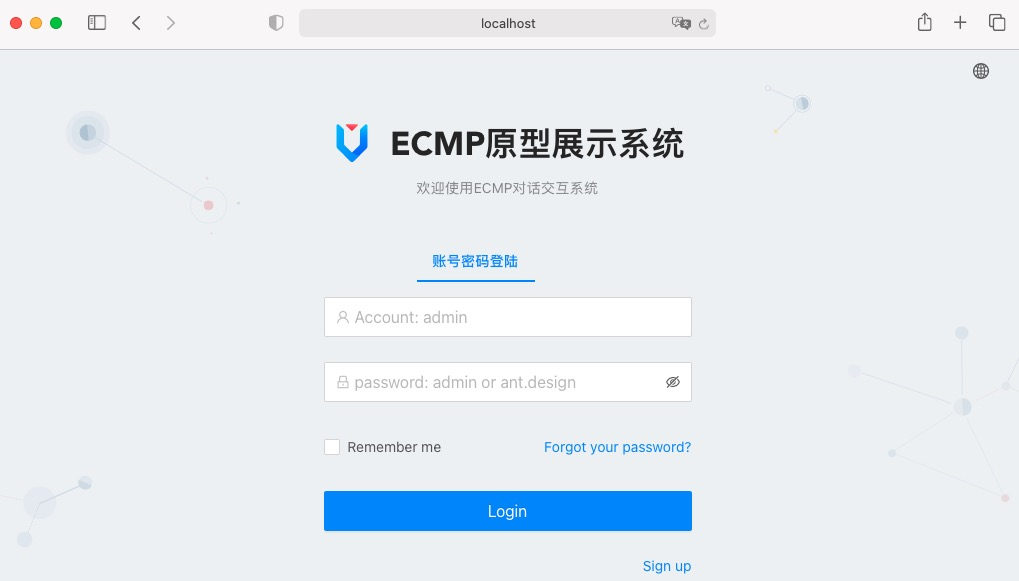
\includegraphics[width=1\textwidth]{images/login.jpg} %插入图片,[]中设置图片大小,{}中是图片文件名
  \caption{交互平台登录页面} %最终文档中希望显示的图片标题
  \label{Fig.login} %用于文内引用的标签
\end{figure}
设计过程中后端主要采用了以下四个API接口:
\begin{itemize}
  \item [1)]auth-login
  \item [2)]get-user-info
  \item [3)]return-2-step-code
  \item [4)]auth-logout
\end{itemize}

分别用于校验用户账号密码、返回用户权限信息、返回登陆状态码以及退出登陆。

而前端则只需要将账号密码字段格式化后通过axios中的post方法将表单传入Django的服务端即可。

\subsubsection{对话互动页面}
如图\ref{Fig.chatbot}所示,侧边栏中一共分为Analysis、Source和ChatBot三个子栏目,分别用于展示数据看板、项目源代码以及对话演示系统。
点击ChatBot即可跳转至ECMP对话系统。
\begin{figure}[H] %H为当前位置,!htb为忽略美学标准,htbp为浮动图形
  \centering %图片居中
  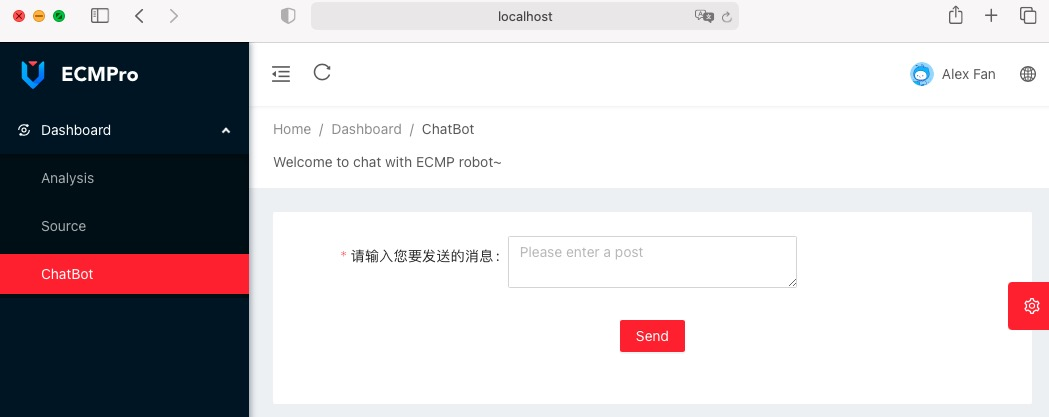
\includegraphics[width=1\textwidth]{images/Chatbot.jpg} %插入图片,[]中设置图片大小,{}中是图片文件名
  \caption{对话互动页面} %最终文档中希望显示的图片标题
  \label{Fig.chatbot} %用于文内引用的标签
\end{figure}

因为本个项目中只涉及单轮对话,所以在对话形式上选择了表单发送的单轮传输模式。在“请输入您要发送的消息”之后传入要输入的语句,并点击“Send”按钮,
即可将会话框中的消息传入后端的ECMP原型系统中,并等待生成response。

如下图\ref{Fig.chatpost}所示,在对话框中输入“今天吃了好吃的”,并通过vue封装好的axios API中的post方法将表单中的语句发送到ECMP系统中。
\begin{figure}[H] %H为当前位置,!htb为忽略美学标准,htbp为浮动图形
  \centering %图片居中
  \includegraphics[width=1\textwidth]{images/chatpost.jpg} %插入图片,[]中设置图片大小,{}中是图片文件名
  \caption{对话互动页面} %最终文档中希望显示的图片标题
  \label{Fig.chatpost} %用于文内引用的标签
\end{figure}

在经过ECMP的情感预测和回复生成之后,得到最佳的回复结果,并通过response将结果返回至前端,并在modal结构中进行打印。如图\ref{Fig.chatresponse}中
原型系统给出的最佳回复为:“看起来很好吃的样子”。
\begin{figure}[H] %H为当前位置,!htb为忽略美学标准,htbp为浮动图形
  \centering %图片居中
  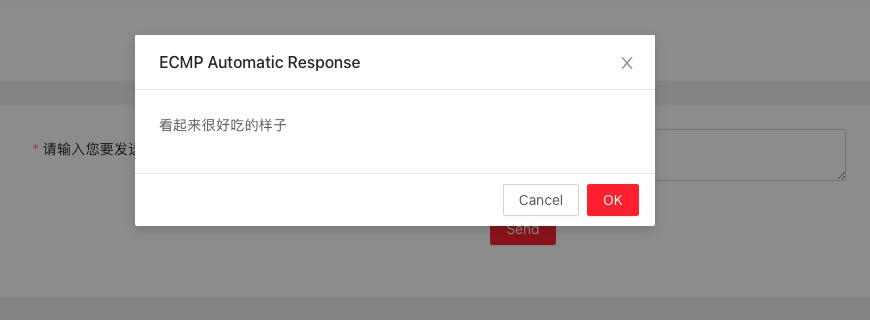
\includegraphics[width=1\textwidth]{images/chatresponse.jpg} %插入图片,[]中设置图片大小,{}中是图片文件名
  \caption{对话互动页面} %最终文档中希望显示的图片标题
  \label{Fig.chatresponse} %用于文内引用的标签
\end{figure}

\subsection{本章小结}
最终的评估结果证明,ECMP模型目前优于现有的所有情感对话模型,因为其拥有情感自动选择器,可以生成更为贴近于真实日常对话中的情感表达。
在风格一致性以及情感一致性上,ECMP也取得不错的成绩。
在之前的情感对话生成中,回复中所嵌入的情感都是单一的情感,但是人类对于情感的感知十分微妙,在言语中所包含的情感也不是只有一个种类,
所以ECMP中提出了情感向量空间并且假定情感概率的分布在整个向量空间上,从而使得生成的回复不会被单一的情绪所约束。

而为了使得本项目能体现其工程化的能力,所以在最后也在原型系统的基础上基于Vue.js和Django设计了一整套便捷的交互界面ECMPro,用于让用户
直观的感受到情感对话生成系统的能力。


\section{总结与展望}
\subsection{个人总结}
总结来说,本次课题也基本上涵盖了我大学四年的主要技术栈,包括python、git、TensorFlow、django以及Vue.js。因为本人比较偏向于工程化项目,但是在深度学习课题中偏向于科研方向,所以在最后也
是做了一些工程化的展示界面,其中使用到了Vue.js技术和Django框架,这些都是目前比较热门的前后端框架,也是在公司实习过程中所做的技术储备。非常幸运的是能在本次课题中有所用武之地。

从代码管理的角度来看,git作为版本管理的头号热门工具,理所应当成为了本项目的版本管理工具。而一直以来GitHub是首选的代码版本管理平台,所以本次课题的所有commit版本都保存在本人的Github仓库中。

而因为本次课题为对话生成相关的课题,在代码实现方面也主要使用到TensorFlow框架,不过由于原生的ECM框架的TensorFlow版本过低,导致了许多新版本的功能不兼容的问题,所以在本次课题结束后,
将准备使用TensorFlow2.0以上版本对项目进行重构,此外整个对话系统的生成和展示都按照预期效果顺利完成。

从工程能力上说,曾经因为没有做过算法类的大型项目,所以本次课题对我也是一个非常大的挑战,而最后的展示系统也是一个纯粹的工程类项目,展示系统的存在让功能更加多样化且交互更加友好。因为不涉及
数据库的开发,在开发成本上不会特别难以接收。并且新系统有比较优秀的可维护性所以在不同的系统上的可兼容性会比较好。

\subsection{未来展望}
对于本课题的未来发展前景,可以非常明显的发现此次课题中不包含知识图谱的构建,所以会导致回复中并没有特别多新颖的信息,在联想方面也有所欠缺,所以在下一个阶段,希望可以构建
ECMP专属的知识图谱来进行基于主题风格化的情感对话系统的构建。此外对于情感对话机器人,独特的人物身份和人物性格的嵌入也会使得人机对话的体验大大提升,而非千篇一律的服务型人格。

TensorFlow的兼容性也是一个比较大的挑战,在之前的ECM项目中,距离开发者的上一次提交已经是4年之前,TensorFlow的版本也非常老旧所以导致现在的维护和扩展成本非常大,所以
下一步的主要工作将会主要围绕在使用TensorFlow2.x来改写原版TensorFlow0.12的原始系统。

对于目前的交互系统,因为没有上线服务器,所以只能在本地局域网运行。在之后可以将整个交互系统上架为合法备案的网站应用并申请相关的域名,更高阶的目标是将其抽象出对话生成API来提供给其他用户更方便地
使用和调用。


\begin{thankpage}
感谢父母的生养和陪伴给予我爱与力量,在他们的勤劳与呵护下,给我构筑了一个美满幸福和谐的家庭,愉快的度过21年的求学时光。

感谢魏巍导师在整个课题研究过程中的悉心指导,众多颇有深度的理念,让我沉浸于研究性课题的魅力。

感谢爱人张雨佳同学一路以来的支持和信任,每个温柔的拥抱给予了莫大的慰藉与安慰,期待同她的美好未来。

感谢恩师杜晓燕老师的启发和鼓励,让我从一个内向笨拙的学生,逐渐充满自信翻转人生。

感谢发小宋梓贤与我相伴成长嬉笑打闹的十余年时光,激发了我对这个世界最初的好奇和探索。

感谢亲朋好友在每个重要阶段的帮助和勉励,深刻感念于家人的温暖。

感谢三位室友同我分享这大学四年里的诸多美好,教会我上进与成长,同低谷,共奋进。

感谢母校华中科技大学及计算机科学与技术学院,让我从一个计算机小白变成今日模样,从一个初生牛犊到如今的但当涉猎。

\end{thankpage}

\nocite{*}

\bibliography{main}

\end{document}
